%-----<<< RESULTS >>>-----
\chapter{Results}
\label{ch:results}

This section presents the findings and results of our research. First, the MAS as described in Chapter~\ref{ch:approach} Figure~\ref{fig_agents} was implemented. After testing the MAS in the simulator (described in Section~\ref{sec-sim}), it was deployed on the actual robot. In order to do that, we had to check the functionality of the hardware. After several tests, it turned out that the moments of inertia of the robot were too large given the size of wings and magnitude of forces and moments they generated. As a result, the robot wasn't agile enough for our size of the water tank -- in other words, the experimental area we had was too small for testing. Since increasing the size of the test area was not feasible, we resolved the problem by making a second version of the robot, and significantly reduced its weight and size. We were able to decrease the weight of the robot by 55\% (from 406~g to 180~g), and the diameter by 30\%, all by optimizing the mechanical and electrical components. The actuators and the wings were unchanged. The second version of the robot had significantly lower moments of inertia, and as a result was much swifter. For more details about the robots we would refer the reader to Appendix~\ref{a:mechanical-design}. 

The next step was to find good $\delta$ and $\omega$ values for maneuvers described in Table~\ref{tab-cmd}. The robot's hardware limits max value of $\omega$ to 30~[rad/s] (minimum is 1~rad/s), and $\delta \in (-10,10)$~[rad/s], while the split-cycle control requires $|\delta|\le \omega/2$ (see Section~\ref{sec-splitCycleControl} for more details), so these values were used as lower and upper bounds for randomly initialized individuals in the (1,10)-ES algorithm (described in Section~\ref{subsec-FirstStageAdaptation}). The strategy parameters were empirically determined to be $\sigma_i \in (3,6)$ where $i={1,2,3,4}$.

As mentioned before, in this phase of the research effort, we used an evolutionary algorithm to search for the optimal values of $\delta$ and $\omega$. Other optimization algorithms might be useful but whether or not that is true would require a detailed analysis of the solution space morphology which we did not do\footnote{However, our experiments did show small perturbations in $\delta/\omega$ had no observed behavioral changes which suggests gradient-based optimization algorithms would not be very effective.}.

Our choice of an evolutionary algorithm to conduct the search was two-fold. First, evolutionary algorithms are usually considered optimization algorithms but basically they are search algorithms. Evolutionary algorithms can search any solution space regardless of morphology. Thus evolutionary algorithms allow us to optimize without conducting a solution space analysis. Secondly, and more importantly, every vehicle is slightly different due to inherent nonlinearities in the linkages and other manufacturing differences (such as a slightly different size of wings, etc.). As a result, \textit{optimal} values for one vehicle will not be optimal for another. The goal here is not to achieve generally optimal movements but rather smooth and repeatable correct movements. Consequently, we needed a search method rather than an optimization method. Evolutionary algorithms allow us to search for good solutions by evaluating actual vehicle behavior, which cannot be accomplished using classical optimization algorithms. Two types of evolution - \textit{extrinsic} and \textit{intrinsic} were used, as described below.

\section{Extrinsic Evolution}
\label{subsec-extrinsic}
Because the lifespan of linkages at the vehicle is limited, it is reasonable to first execute extrinsic evolution of control parameters $\delta$ and $\omega$ to 1) verify the correctness of the evolution algorithm; 2) get the initial estimate of satisfactory control parameters. A more precise model of the vehicle produces a better estimate. However, obtaining a precise (first-principle) model of the flapping wing system is very complicated, especially because of the small forces and torques that would have to be measured to correctly identify the model~\cite{Finio2011}. Modelling non-linearities such as linkage slip also poses a significant challenge~\cite{Vm2015}. However a simplified model that treats the vehicle as a point mass body and aggregates the generated forces and torques is a sufficient approximation, because it will exhibit similar behavior albeit on a different time scale.

For the purpose of the extrinsic evolution, we started with the following assumption. The faster the wings beat (i.e. higher $\omega$), the more force is generated (because the wing acceleration is higher). The higher split cycle shift (higher $|\delta|$), the more force is generated (because the difference between upstroke and downstroke is higher). The higher force results into faster movement.

The best solution completes the basic movement in the shortest time, and is within the imposed constraints. Thus in our simple model we use to evaluate fitness of candidate solution we employ the following equation:
\begin{equation}
\textrm{fit}(x) = K_L \cdot \delta_{L_x} \cdot \omega_{L_x} + K_R \cdot \delta_{R_x} \cdot \omega_{R_x}
\end{equation}

where $K_L, K_R$ are adjustable weights, in the simplest case:
\begin{itemize}
\item $K_L = K_R = 1$ for \textit{Move forward}
\item $K_L = 1; K_R = -1$ for \textit{Turn right}
\item $K_L = -1; K_R = 1$ for \textit{Turn left}
\end{itemize}

We ran the EA for 20 generations in each run, for 20 runs total. The expected optimal solution would converge to maximal $\omega$ for both wings and maximal values for $\delta$ but with opposite signs in case of turns. The results are shown in Figure~\ref{fig-extrinsic}. Notice in all cases the runs converged to (or at least very close to) the global optimum. 
The best evolved values for our simple model are summarized in Table~\ref{tab-ctrl-values-extrinsic}, and they are consistent with our expectations.


\section{Intrinsic Evolution}
\label{subsec-intrinsic}
During the intrinsic evolution we used the actual vehicle for evaluating fitness of the candidates. The major difference was that for \textit{Turn left} and \textit{Turn right} fitness is defined as $f=1/T$ where $T$ is the time needed for the vehicle to turn by 360 degrees from its initial position. For \textit{Move forward} the fitness is defined as $f=1/(\alpha \cdot T_{wp} + \beta \cdot d_{wp})$, where $T_{wp}$ is time needed to reach x-coordinate of the waypoint \textit{p} (located approximately 30~cm in front of the vehicle), $d_{wp}$ is the distance from the y-coordinate of the waypoint \textit{p} when its x-coordinate is reached. $\alpha = 100$ and $\beta = 1$ are weights to scale the different units (seconds and pixels). 

Because the hardware has a limited lifespan, we only ran the EA once and for only 20 generations. This is limiting in the sense that we can reach suboptimal results, but if we were to run more runs as was the case for extrinsic evolution, the linkages could wear out prematurely and would have to be replaced, in which case the learning would have to be done again from the beginning. %In other words, extrinsic evolution provides relatively good results, but to obtain a fine-tuned control system we need to use intrinsic evolution.

The incremental improvements in turn times for evolved control parameters are shown in Figure~\ref{fig-intrinsic}. For the forward motion, the vehicle actually was not able to reach the desired waypoint (its $y$-coordinate) in vast majority of tries. In such case the experiment was stopped after 2 minutes and the fitness of given individual was marked as zero. Effectively this reduced the EA to a random search, until a viable solution was found. The best solution after 20 generations (and the only one found that had non-zero fitness) is shown in Figure~\ref{fig-intrsc-fw}. The best values of control parameters found for our vehicle are summarized in Table~\ref{tab-ctrl-values-intrinsic}. The best intrinsically evolved values are very similar to the values found by extrinsic evolution (compare with Table~\ref{tab-ctrl-values-extrinsic}). This validates the model used for extrinsic evolution, and makes it usable for the initial estimate. The differences in control parameters are caused by imperfections and non-linearities in real hardware, and indeed, those were not included in our model. The intrinsically evolved values, recorded in Table~\ref{tab-ctrl-values-intrinsic}, were used for further experiments.

\begin{figure}
\centering
\minipage{0.49\textwidth}
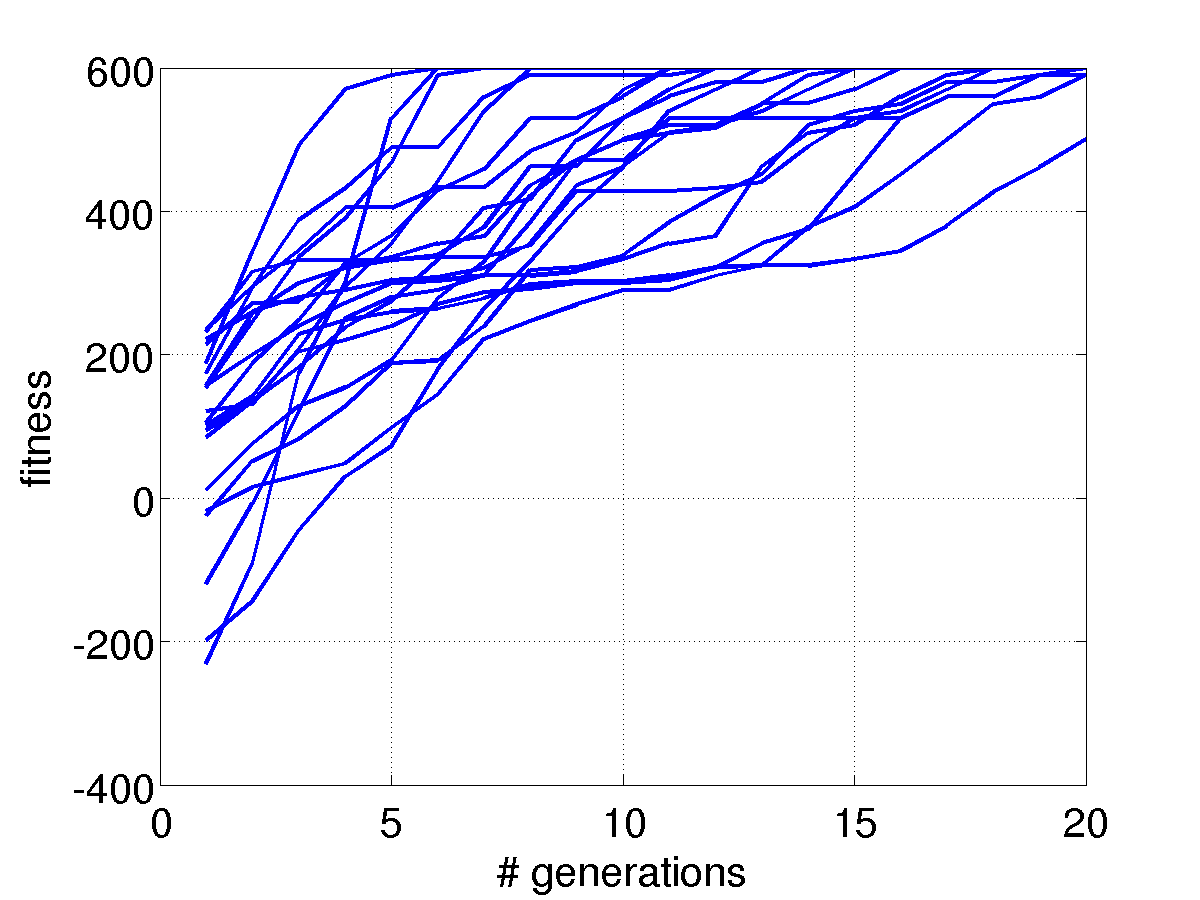
\includegraphics[width=\textwidth]{Files/Figures/extrinsic.png}
\caption[Extrinsic evolution run for \textit{Turn left} move]{Extrinsic evolution run for \textit{Turn left} move. Notice that the algorithm in almost all cases reaches global optimum $f=600$ \newline \newline}
\label{fig-extrinsic}
\endminipage\hfill
\minipage{0.49\textwidth}
\centering
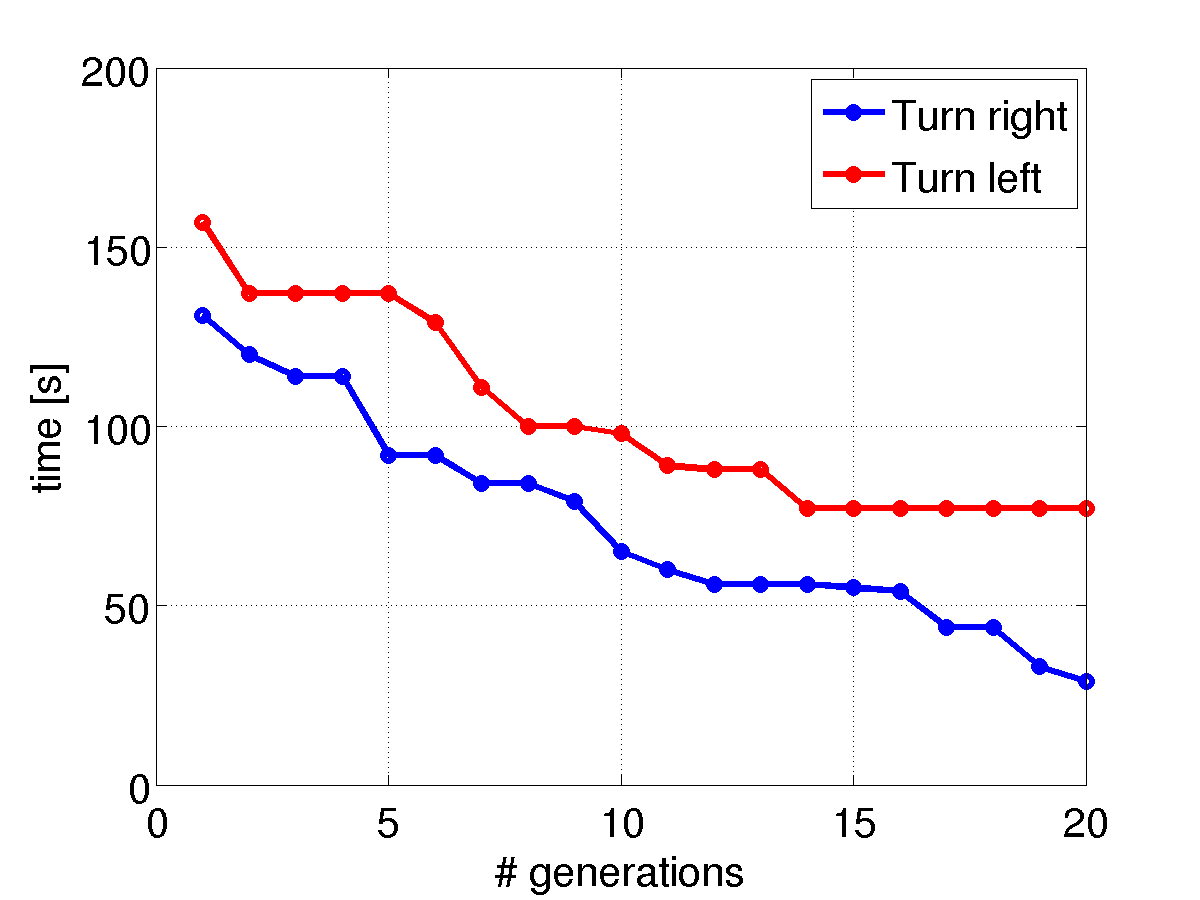
\includegraphics[width=\textwidth]{Files/Figures/intrinsic.png}
\caption[Intrinsic evolution run for \textit{Turn left} and \textit{Turn right} moves]{Time needed to complete \textit{Turn left} and \textit{Turn right} moves during intrinsic evolution. Notice that left turn takes longer to finish, which is caused by non-linearities in the hardware. The fitness is inversely proportional to the turn times.}
\label{fig-intrinsic}
\endminipage\hfill
\end{figure}


\begin{figure}
\centering
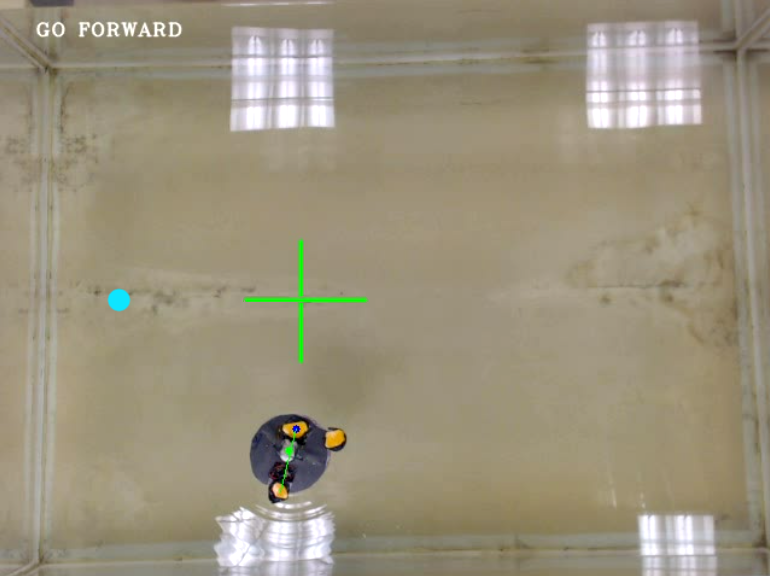
\includegraphics[width=0.75\textwidth]{Files/Figures/go_fw.png}
\caption[Best found solution for forward movement]{Best found solution for forward movement \textit{Blue:} Initial position of the vehicle, \textit{Green cross:} waypoint the vehicle was commanded to reach. The experiment was stopped once the center of vehicle crossed the $y$-axis of the waypoint. The four white rectangles are reflections of the ceiling lights and are not related to the experiment.}
\label{fig-intrsc-fw}
\end{figure}

\begin{table}
\centering
\minipage{0.49\textwidth}
\renewcommand{\arraystretch}{1.7}
\begin{tabular}{l|cccc}
\hline
\multirow{2}{*}{Movement} & $\delta_L$ & $\delta_R$ & $\omega_L$ & $\omega_R$  \\
  & \multicolumn{4}{c}{[rad/s]}\\
\hline
\rowcolor{Gray}
Move Forward & \textbf{10} & \textbf{10} & \textbf{30} & 30 \\
Left Turn & \textbf{-10} & 10 & \textbf{30} & 30 \\
\rowcolor{Gray}
Right Turn & 10 & -10 & 30 & 30 \\
Idle & 0 & 0 & 0 & 0 \\
\hline
\end{tabular}
\newline
\caption[Control parameters for the basic movements - extrinsic evolution]{Control parameters for the basic movements obtained from extrinsic evolution. The values that differ from those obtained by \textit{intrinsic evolution} are bold. Values for \textit{Idle} (which simply stops the actuators) were not evolved. \newline \newline}
\label{tab-ctrl-values-extrinsic}
\endminipage\hfill
\minipage{0.49\textwidth}
\renewcommand{\arraystretch}{1.7}
\begin{tabular}{l|cccc}
\hline
\multirow{2}{*}{Movement} & $\delta_L$ & $\delta_R$ & $\omega_L$ & $\omega_R$  \\
  & \multicolumn{4}{c}{[rad/s]}\\
\hline
\rowcolor{Gray}
Move Forward & \textbf{12} & \textbf{14} & \textbf{25} & 30 \\
Left Turn & \textbf{0} & \textbf{12} & \textbf{12} & 30 \\
\rowcolor{Gray}
Right Turn & \textbf{12} & \textbf{0} & \textbf{25} & \textbf{12} \\
Idle & 0 & 0 & 12 & 12 \\
\hline
\end{tabular}
\newline
\caption[Control parameters for the basic movements - intrinsic evolution]{Control parameters for the basic movements obtained from intrinsic evolution. Values for \textit{Idle} were determined empirically and based on the hardware initialization procedure (default values). The values for \textit{Left Turn}, \textit{Right Turn}, and \textit{Move Forward} differ from those obtained by \textit{extrinsic evolution} are bold.}
\label{tab-ctrl-values-intrinsic}
\endminipage\hfill
\end{table}

\newpage

\section{Waypoint Following}
\label{sec-wp-follwing}

Once the control parameters for the basic moves were learned, it was possible to proceed towards waypoint following. Two waypoints were placed to the opposite sides of the water tank, and the vehicle was expected to go back and forth between them. Two waypoints were sufficient because following them required all basic maneuvers. The vehicle was able to follow successfully the waypoints, as can be seen in Figures~\ref{fig-wp-follow} and \ref{fig_wp_plot}. The vehicle is as large as the dotted circle shown around waypoints in Figure~\ref{fig_wp_plot}, so once the center of the vehicle reaches the dotted circle, the waypoint is considered to be reached. Figure~\ref{fig:wp_control_inputs} shows control inputs and rules that fired during the experiment. We can see that all three rules (\textit{Turn Left}, \textit{Turn Right}, \textit{Go Forward}) are used a similar amount of time. Figure~\ref{fig:wp_orientation} shows the heading of the vehicle (there is a wrap-around at 180 and -180~deg). We can see that the heading is relatively steady, changing between $\sim10$ degrees and $\sim-170$ degrees as the vehicle goes back and forth between the waypoints. The spikes indicate turn-arounds after reaching the waypoints. The rate of change is within $\pm10$~[deg/s] during the whole experiment, as shown in Figure~\ref{fig:wp_ang_rate}. This indicates that the vehicle is moving as fast as possible and that its dynamics are relatively slow.

\begin{figure}
\centering
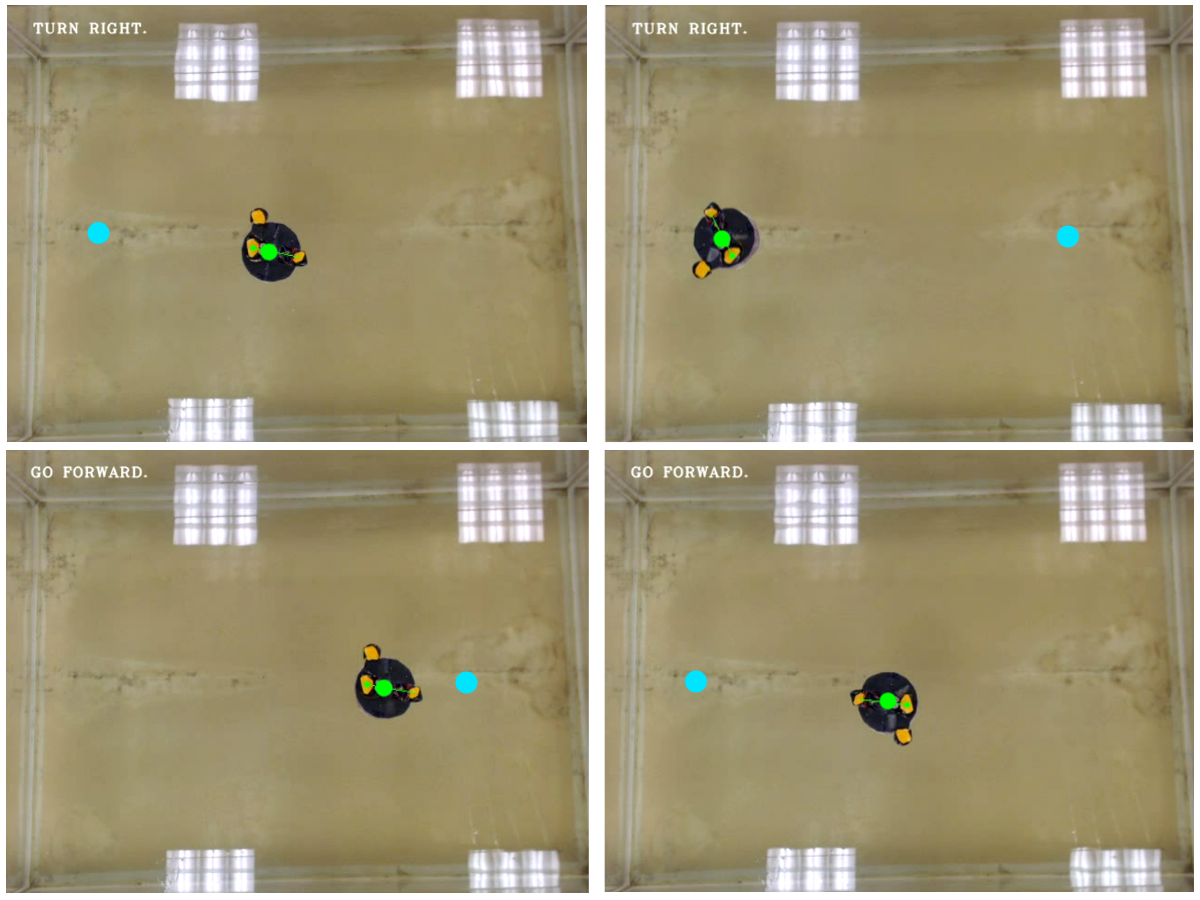
\includegraphics[width=\textwidth]{Files/Figures/wp_example.png}
\caption[Autonomous waypoint following]{Autonomous waypoint following. The blue dot is the desired waypoint; the vehicle is marked with a bright green dot and a green line pointing towards the front of the vehicle. In the top left corner of the screen is shown the rule that fired. Top left: Initial position of the vehicle; Top right: First waypoint achieved, the vehicle is turning around; Bottom left: Approaching the second waypoint; Bottom right: Second waypoint achieved, moving back to the first waypoint.}
\label{fig-wp-follow}
\end{figure}

\begin{figure}
\centering
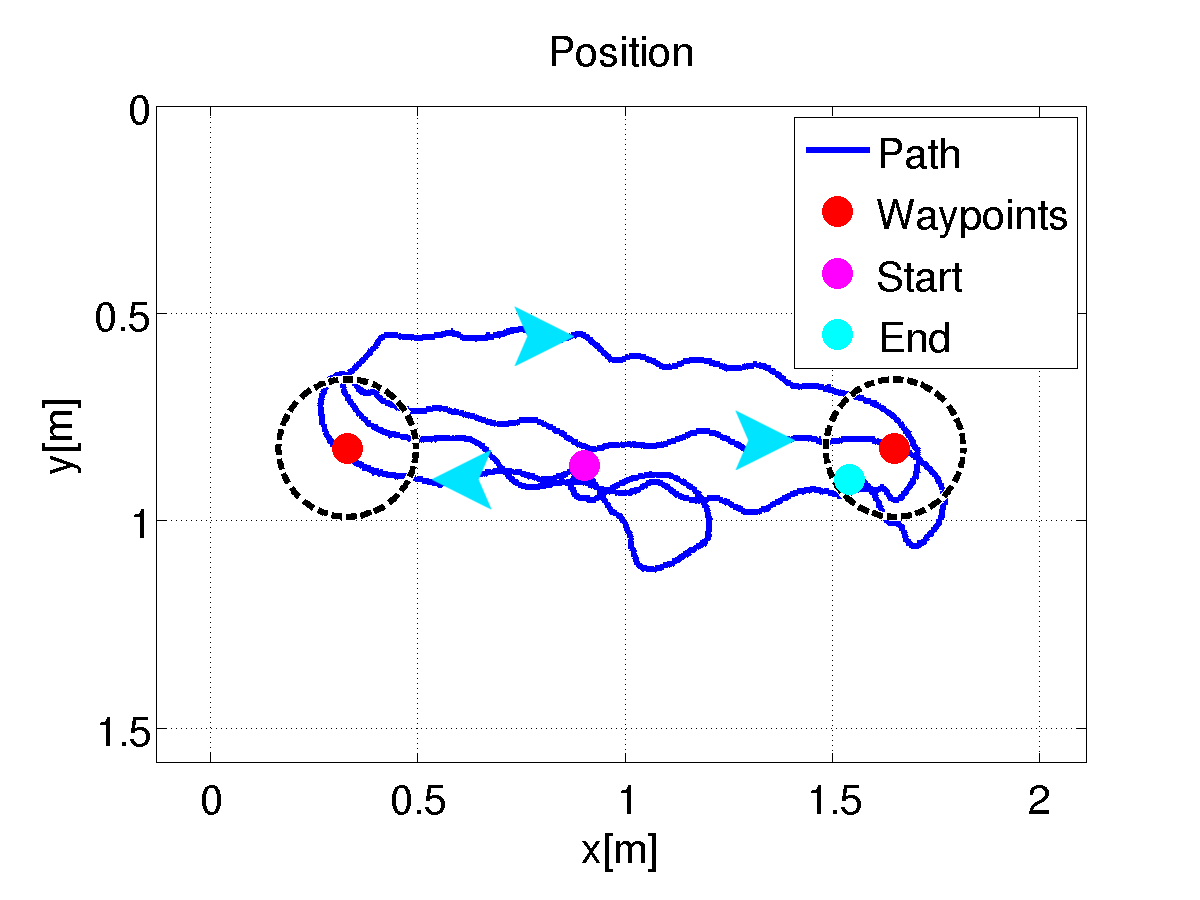
\includegraphics[width=0.8\textwidth]{Files/Figures/wp_2015-10-29_18-42-34-position.png}
\caption[Vehicle trajectory during waypoint following]{Vehicle trajectory (blue) during waypoint following. Two waypoints being followed are marked with red dots, with distance threshold pictured around them. The vehicle itself is as large as the circle around the waypoints. \textit{Purple:} start position, \textit{Light blue:} end position, \textit{Blue arrows:} indicate orientation of the vehicle }
\label{fig_wp_plot}
\end{figure}

\begin{figure}
\centering
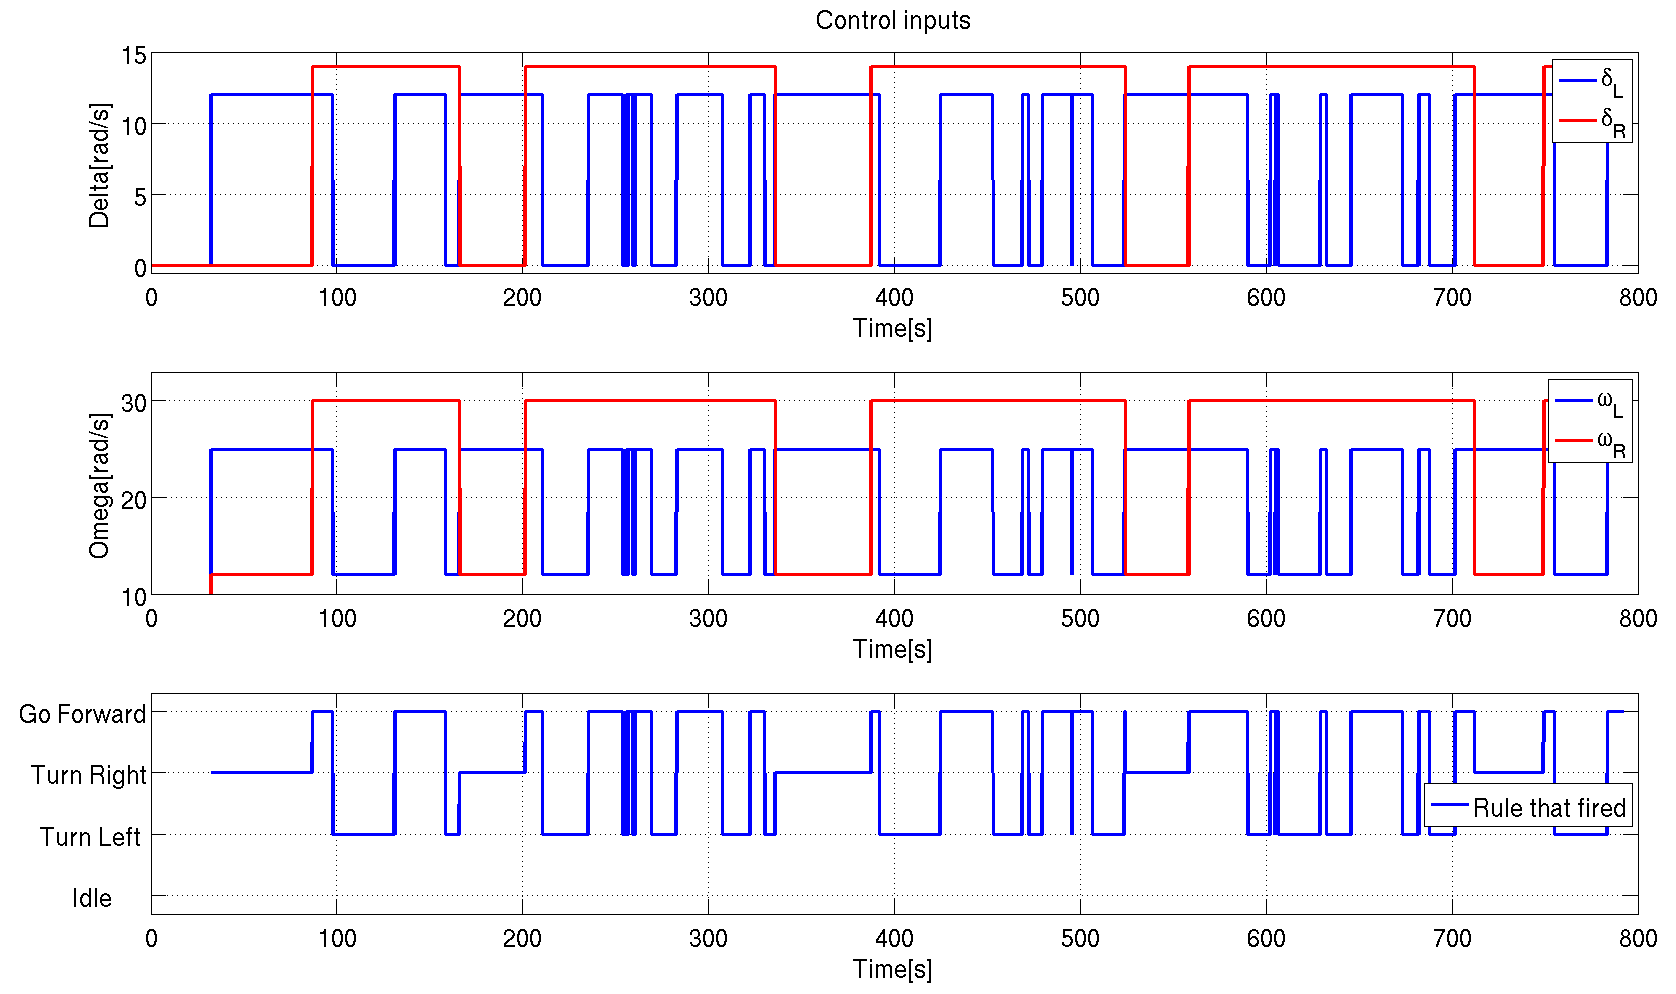
\includegraphics[width=\textwidth]{Files/Figures/wp_2015-10-29_18-42-34-control-inputs.png}
\caption[Control inputs during waypoint following]{Control inputs during waypoint following. \textit{Top:} $\delta$ values, \textit{Middle:} $\omega$ values, \textit{Bottom:} rule that fired.}
\label{fig:wp_control_inputs}
\end{figure}

\begin{figure}
\centering
\minipage{0.49\textwidth}
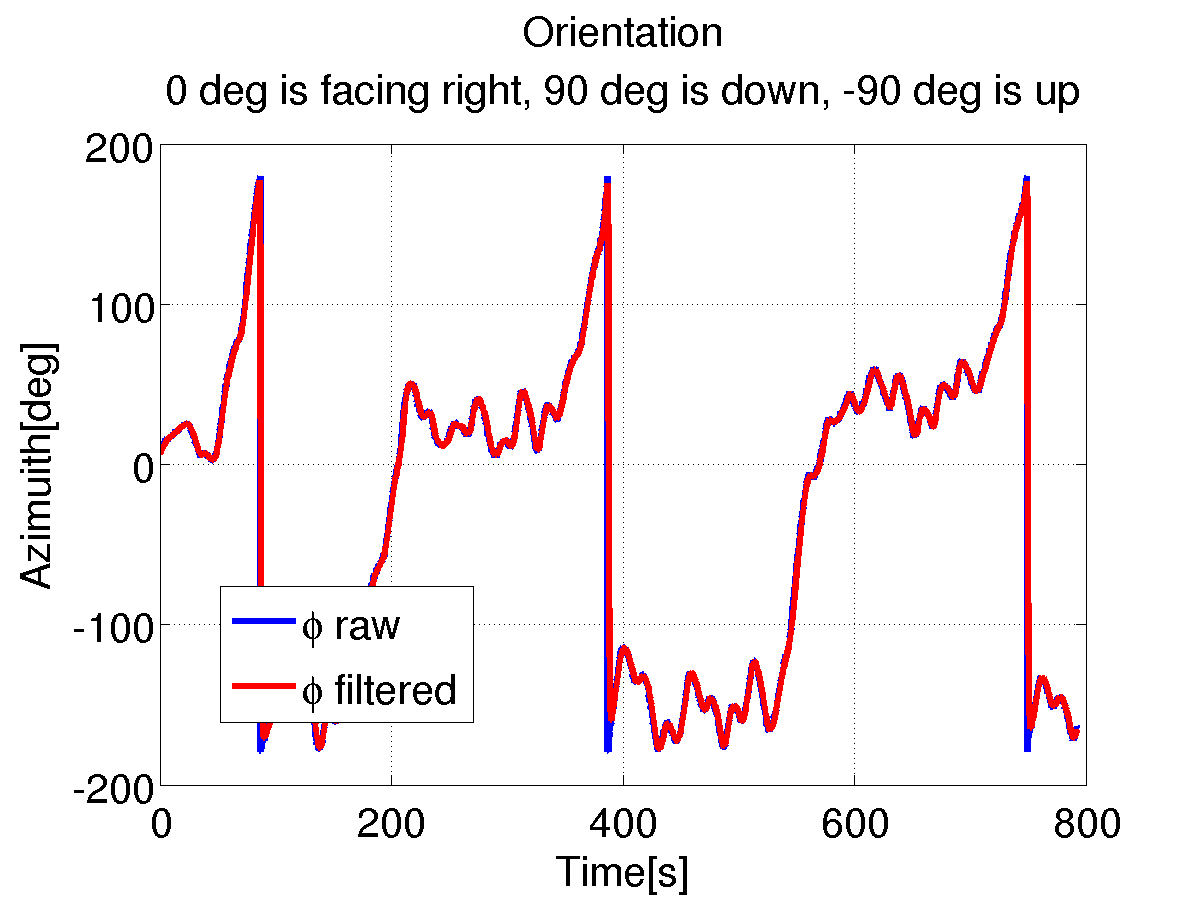
\includegraphics[width=\textwidth]{Files/Figures/wp_2015-10-29_18-42-34-orientation.png}
\caption[Orientation during waypoint following]{Heading of the vehicle during waypoint following. Note the wrap-around at $\pm180$~deg. 0~deg is in the direction of positive x-axis, $\pm180$~deg is in the direction of negative x-axis. The values were filtered with an exponential moving average low-pass filter with $\alpha=0.05$}
\label{fig:wp_orientation}
\endminipage\hfill
\minipage{0.49\textwidth}
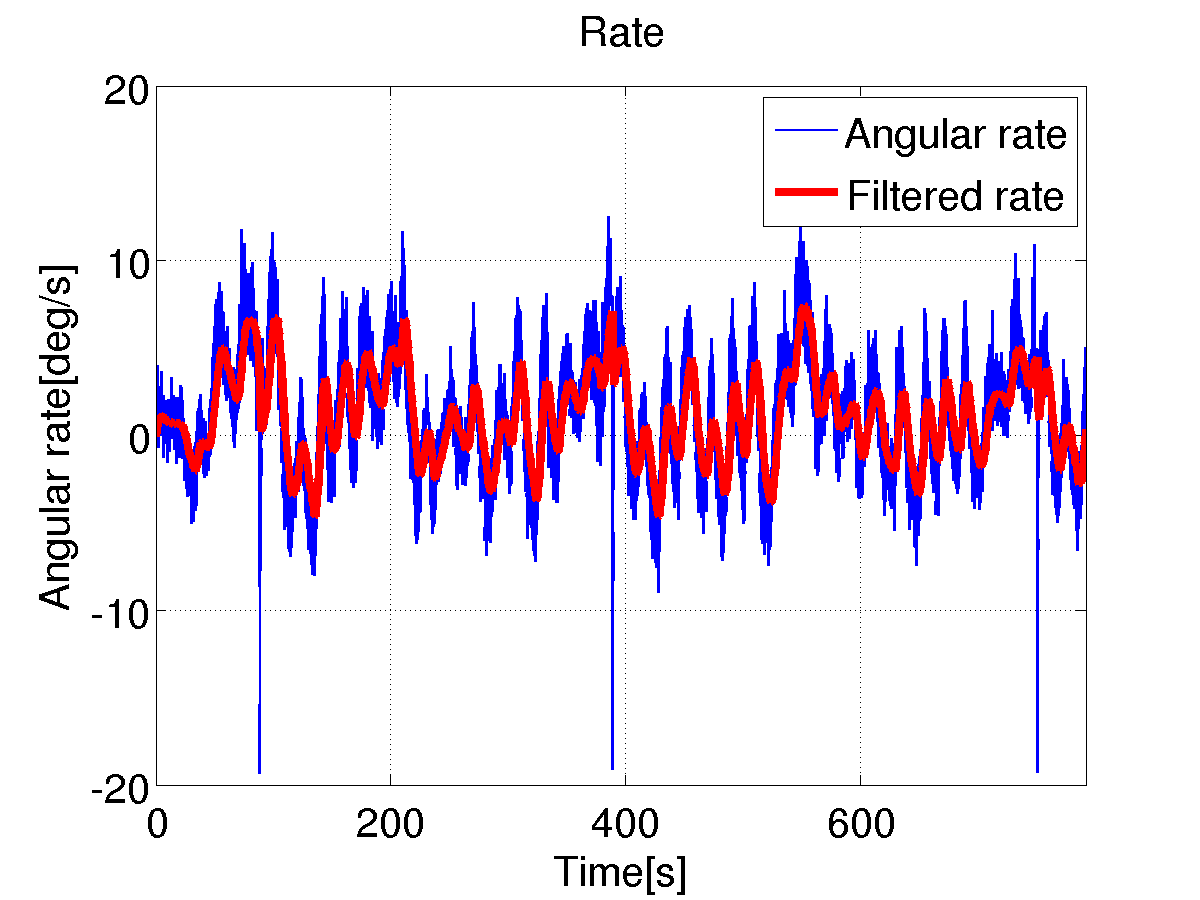
\includegraphics[width=\textwidth]{Files/Figures/wp_2015-10-29_18-42-34-ang_rate.png}
\caption[Angular rate during waypoint following]{Angular rate of the vehicle's heading during waypoint following. The values were filtered with an exponential moving average low-pass filter with $\alpha=0.05$ The peaks are residuals from wrap-arounds at $\pm180$~deg.\newline}
\label{fig:wp_ang_rate}
\endminipage\hfill
\end{figure}


To get a better estimate about the time required to reach a waypoint and to turn left or right, the waypoint following experiment was repeated ten times. The times for each run as well as averaged times are summarized in Table~\ref{tab:times-normal}. We can see that the two waypoints can be reached on average in 5 minutes. The large range (from 2~min 31~seconds to 7~min 2~seconds) is mostly due to varying initial conditions.

We also measured intervals needed for \textit{Turn left} and \textit{Turn right} in order to have a baseline of the robot's performance. Both turns were by 360~deg and were measured ten times from zero initial conditions (i.e. the vehicle wasn't in motion). The results are in Table~\ref{tab:times-normal} which provides data necessary for construction of the pose density function. Figures~\ref{fig:box_turn_left}, \ref{fig:box_turn_right} and \ref{fig:box_waypoint} show the box plots for each of the performed manoeuvres. Box plots show the interquartile range (IQR) between 25th and 75th quartile, IQR hence represents 50\% of the cases (blue box). The median is displayed in red, min and max values are in dashed black. Any outliers (past lower/upper quartile or $\pm2.698\sigma$ interval) are shown in red. These baseline measurements are important for fault recovery mechanism as is shown in the next section.

\begin{table}
\centering
\renewcommand{\arraystretch}{1.0}
\begin{tabular}{rccc}
\hline
\# & Turn Left & Turn Right & Waypoints\\
 & [mm:ss.ss] & [mm:ss.ss] & [mm:ss.ss]\\
\hline
\rowcolor{Gray}
1 & 00:52.00 & 01:53.00 & 05:01.00\\
2 & 00:52.00 & 01:36.00 & 07:02.00\\
\rowcolor{Gray}
3 & 00:42.00 & 01:25.00 & \textit{N/A}\\
4 & 00:46.00 & 01:07.00 & \textit{N/A}\\
\rowcolor{Gray}
5 & 00:39.00 & 01:02.00 & 06:18.00\\
6 & 01:02.00 & 01:15.00 & 05:46.00\\
\rowcolor{Gray}
7 & 00:38.00 & 00:56.00 & 04:33.00\\
8 & 00:45.00 & 01:18.00 & 03:55.00\\
\rowcolor{Gray}
9 & 00:39.00 & 01:13.00 & 06:12.00\\
10 & 01:01.00 & 01:14.00 & 02:31.00\\
\hline
\textbf{Mean:} & \textbf{00:47.00} & \textbf{01:17.90} & \textbf{05:09.75}\\
\textbf{Max:} & 01:02.00 & 01:53.00 & 07:02.00\\
\textbf{Min:} & 00:38.00 & 00:56.00 & 02:31.00\\
\hline
\end{tabular}
\newline
\caption[Basic maneuvers performed under nominal conditions]{Basic maneuvers performed under nominal conditions with control parameters intrinsically evolved. \textit{Turn Left} and \textit{Turn Right} times are for a 360~deg rotation from zero initial conditions. \textit{Waypoints} are two at the opposite sides of the water tank, the vehicle starts at waypoint 1 and the time is running until it reaches Waypoint 2}
\label{tab:times-normal}
\end{table}

\begin{figure}
\centering
\minipage{0.33\textwidth}
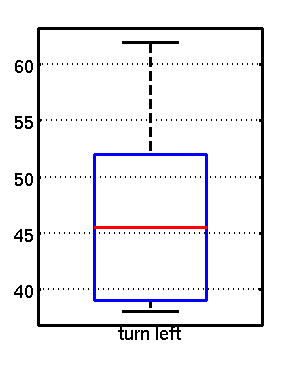
\includegraphics[width=\textwidth]{Files/Figures/box_turn_left.png}
\caption[Box plot of turn left]{Boxplot of \newline \textit{Turn Left} times. \newline
Median: 45.5[s]\newline
25th percentile: 39[s]\newline
75th percentile: 52[s]}
\label{fig:box_turn_left}
\endminipage\hfill
\minipage{0.33\textwidth}
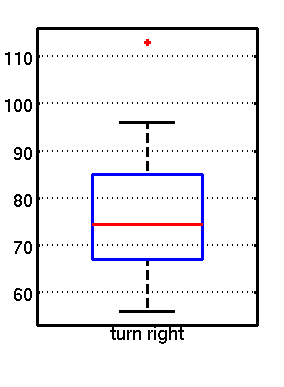
\includegraphics[width=\textwidth]{Files/Figures/box_turn_right.png}
\caption[Box plot of turn right]{Boxplot of \newline \textit{Turn Right} times. \newline
Median: 74.5[s]\newline
25th percentile: 67[s]\newline
75th percentile: 85[s]}
\label{fig:box_turn_right}
\endminipage\hfill
\minipage{0.33\textwidth}
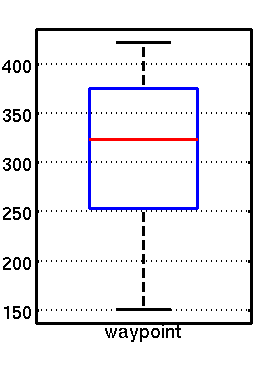
\includegraphics[width=\textwidth]{Files/Figures/box_waypoint.png}
\caption[Box plot of waypoint]{Boxplot of \newline \textit{Waypoint following} times \newline
Median: 323[s] (5:23)\newline
25th percentile: 254[s] (4:14)\newline
75th percentile: 375[s] (6:15)}
\label{fig:box_waypoint}
\endminipage\hfill
\end{figure}

\newpage

\section{Fault recovery}
\label{sec:fault-recovery}

Fault detection and recovery is an important feature, as was mentioned in Chapter~\ref{sec-AgentAdaptation}. Without a loss of generality we set up a fault detection and recovery mechanism for one fault - a damage of the left wing. In a similar manner a damage of the right wing can be detected and consequently recovered. In practice, the damage could occur after a collision with an obstacle. In the experimental setup the wing was cut down by around 30\% (see Figures~\ref{fig:original-wing} and~\ref{fig:damaged-wing-detail}). Because the tip of the wing produces most of the aerodynamic forces, we can expect an even higher loss of performance. After damaging the wing, identical maneuvers as with undamaged wing were performed (i.e. no adaptation of $\delta$ and $\omega$ parameters occurred). The times are recorded in Table~\ref{tab:times-damaged}. Since the left wing was damaged, we expect \textit{Turn Right} turn to be mostly impacted, and as a result waypoint following ability will be affected too. 

\begin{figure}
\centering
\minipage{0.49\textwidth}
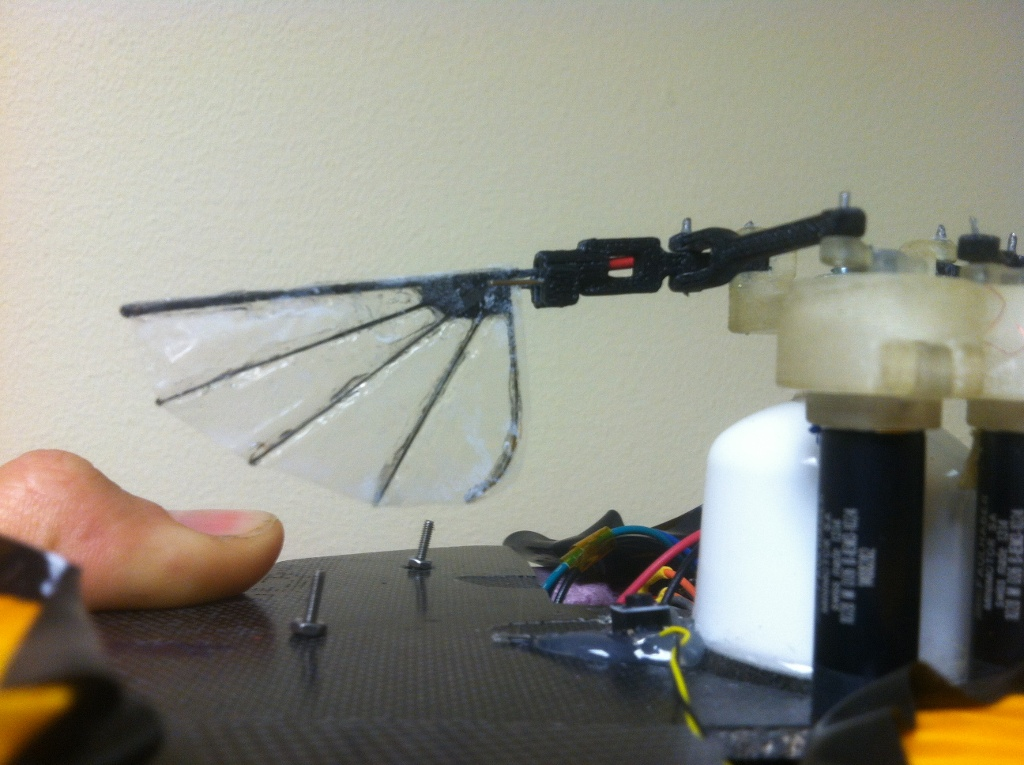
\includegraphics[width=0.9\textwidth]{Files/Figures/photo3.JPG}
\caption[Original Wing]{Detail of the original left wing \newline \newline \newline}
\label{fig:original-wing}
\endminipage\hfill
\minipage{0.49\textwidth}
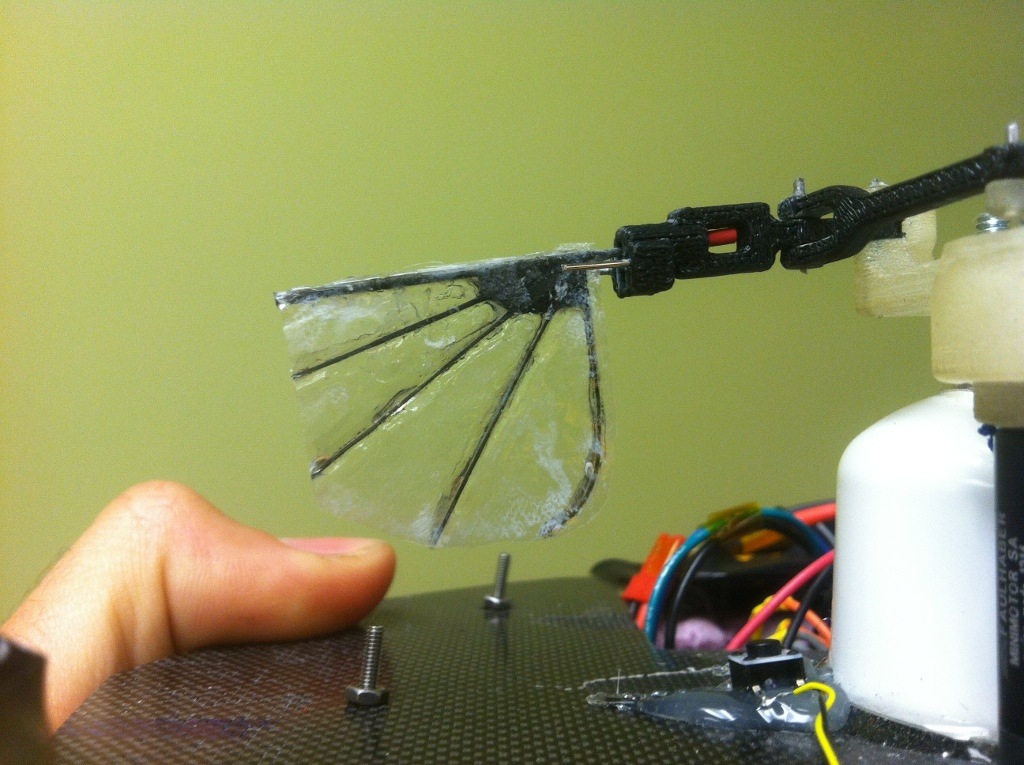
\includegraphics[width=0.9\textwidth]{Files/Figures/photo4.JPG}
\caption[Damaged wing]{Detail of the damaged left wing, roughly 30\% of the surface area was removed \newline}
\label{fig:damaged-wing-detail}
\endminipage\hfill
\end{figure}

For \textit{Turn Right} we observe 44\% increase in the average time to perform the turn (from 1:17 to 1:51), while \textit{Turn Left} is impacted only minimally (increase by 6\% from 00:47 to 00:50 on average). Interestingly, the vehicle is still able to follow the waypoints albeit with worse performance. Note that the waypoint following was executed only once to avoid excessive strain on linkages and premature wear of the vehicle.


In order to detect the fault, the vehicle - after it initializes - performs a 360~deg \textit{Turn Right} and measures the time $T$ it takes. If $T > T_{max}$ where $T_{max}=94$[s], then the \textit{Left Wing Damaged} fault is triggered. We work under a reasonable assumption that the damaged vehicle will not be any faster than during normal operation, hence only $T_{max}$ is considered. The $T_{max}	$ was calculated as $1\sigma$ (standard deviation) from the mean\footnote{Using \textit{median} instead of \textit{mean} for calculating $\sigma$ would be justifiable in this case, because only 10 samples is a fairly low number and thus \textit{median} represents the average value better. As the number of samples increase, \textit{mean} and \textit{median} would become closer and closer. However, the difference of around 4 seconds between the \textit{mean} and \textit{median} times is very insignificant given the slow dynamics of our vehicle.} of the baseline performance of \textit{Turn Right}. One standard deviation covers 68\% of cases, which is a reasonable for our purposes. Figure~\ref{fig:hist_turn_right} shows the histogram of \textit{Turn Right} times as well as the standard deviation. Indeed the distribution is normal. 

To recover from the fault, we had to again intrinsically evolve the $\delta$ and $\omega$ parameters. Note that the initial assumption was that this fault is recoverable - i.e. with a proper control input full function of the vehicle is possible. Other faults, for example a broken linkage or a stuck motor would not be recoverable. We run the ES algorithm in the same way as for determining the original values (see Section~\ref{subsec-intrinsic} for details). After running the intrinsic evolution for 20 generations the evolved $\delta$ and $\omega$ values were stored in Table~\ref{tab-ctrl-values-recovered}.

Once the recovery values were found, it was possible to test their effect. The average times as well as individual trial times for all the basic maneuvers are shown in Table~\ref{tab:times-repaired}. With the updated control values the times for \textit{Turn Left} and \textit{Turn Right} are comparable with the undamaged wings, and so is the waypoint following. Once again, to conserve the hardware only two iterations of waypoint following were performed. Figure~\ref{fig:fault_recovery_pics} shows the fault recovery experiment, Figure~\ref{fig:fault_recovery_path} shows the tracked path of the vehicle, and Figures~\ref{fig:fault_recovery_orientation} and ~\ref{fig:fault_recovery_ang_rate} show the orientation and angular rates of the vehicle. The control inputs are shown in Figure~\ref{fig:fault_recovery_control_input}, the long period of \textit{Turn Right} at the beginning of the experiment is when the diagnostics agent is running the test for presence of a fault. In a similar fashion \textit{Right Wing Damaged} fault could be detected and recovered from, assuming only one fault occurs at a time. Figure~\ref{fig:box_recovery} compares the \textit{Turn Right} times between original, damaged and recovered conditions. We can clearly see that the recovered turn time is comparable to the original time (within interquartile range or $\pm0.6745\sigma$), and as a result the fault recovery was successful.

\begin{table}
\centering
\renewcommand{\arraystretch}{1.0}
\begin{tabular}{rccc}
\hline
\# & Turn Left & Turn Right & Waypoints\\
 & [mm:ss.ss] & [mm:ss.ss] & [mm:ss.ss]\\
\hline
\rowcolor{Gray}
1 & 00:45.00 & 02:12.00 & 06:15.00\\
2 & 00:51.00 & 01:42.00 & \textit{N/A}\\
\rowcolor{Gray}
3 & 01:14.00 & 01:39.00 & \textit{N/A}\\
4 & 00:48.00 & 01:25.00 & \textit{N/A}\\
\rowcolor{Gray}
5 & 00:44.00 & 01:18.00 & \textit{N/A}\\
6 & 00:55.00 & 01:55.00 & \textit{N/A}\\
\rowcolor{Gray}
7 & 00:42.00 & 01:43.00 & \textit{N/A}\\
8 & 00:42.00 & 02:12.00 & \textit{N/A}\\
\rowcolor{Gray}
9 & 00:49.00 & 02:24.00 & \textit{N/A}\\
10 & 00:49.00 & 02:03.00 & \textit{N/A}\\
\hline
\textbf{Mean:} & \textbf{00:50.00} & \textbf{01:51.30} & \textbf{06:15.00}\\
\textbf{Max:} & 01:14.00 & 02:24.00 & \textit{N/A}\\
\textbf{Min:} & 00:42.00 & 01:18.00 & \textit{N/A}\\
\hline
\end{tabular}
\newline
\caption[Basic maneuvers performed after wing damage]{Basic maneuvers performed after left wing damage (control parameters unchanged).}
\label{tab:times-damaged}
\end{table}


\begin{table}
\centering
\renewcommand{\arraystretch}{1.7}
\begin{tabular}{l|cccc}
\hline
\multirow{2}{*}{Movement} & $\delta_L$ & $\delta_R$ & $\omega_L$ & $\omega_R$  \\
  & \multicolumn{4}{c}{[rad/s]}\\
\hline
\rowcolor{Gray}
Move Forward & \textbf{14} & 14 & \textbf{30} & 30 \\
Left Turn & 0 & \textbf{14} & 12 & 30 \\
\rowcolor{Gray}
Right Turn & \textbf{14} & 0 & \textbf{30} & 12 \\
Idle & 0 & 0 & 12 & 12 \\
\hline
\end{tabular}
\newline
\caption[Evolved fault recovery control parameters]{Evolved fault recovery control parameters. Values for \textit{Idle} were determined empirically and based on the hardware initialization procedure (default values). The values for \textit{Left Turn}, \textit{Right Turn}, and \textit{Move Forward} differ from the undamaged values are bold.}
\label{tab-ctrl-values-recovered}
\end{table}

\begin{figure}
\centering
\minipage{0.49\textwidth}
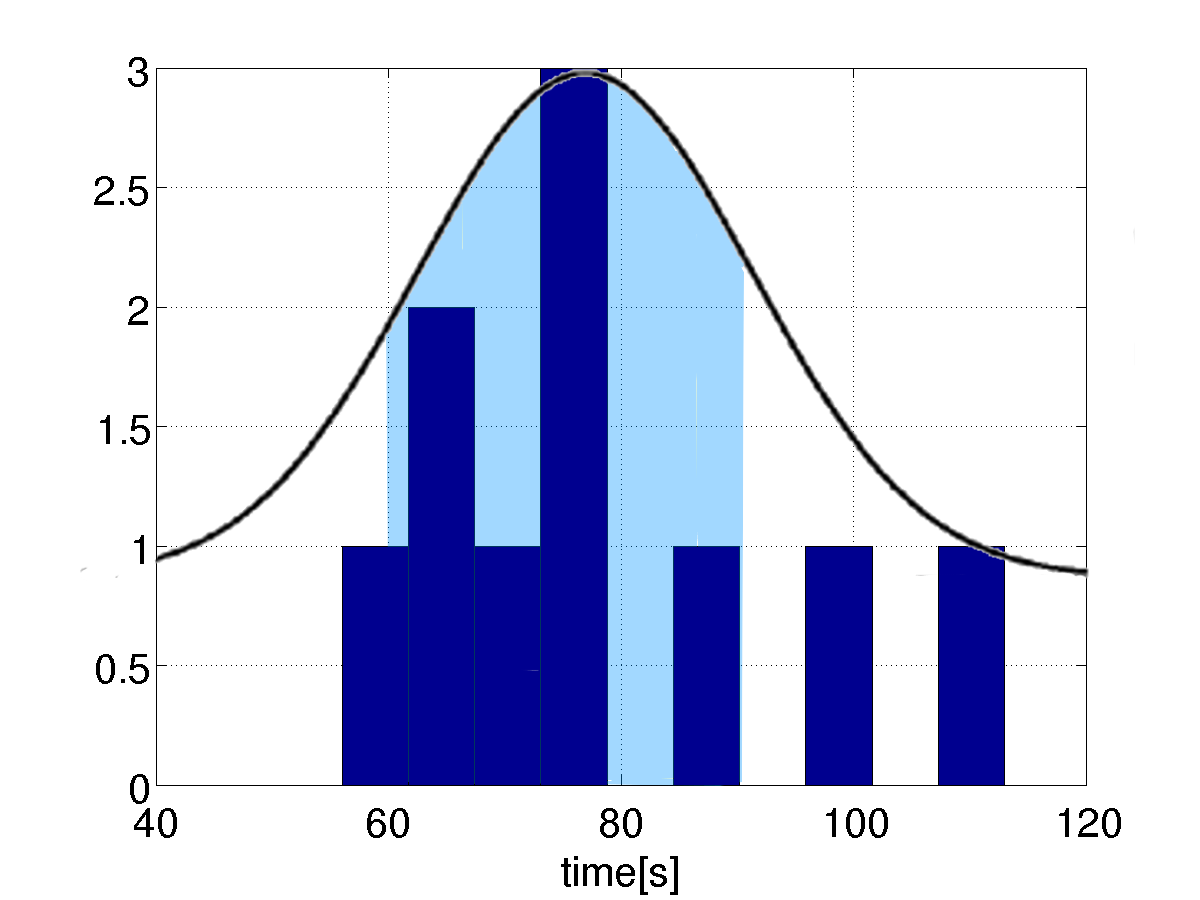
\includegraphics[width=\textwidth]{Files/Figures/hist_turn_right.png}
\caption[Histogram of turn right move]{Histogram of the original \textit{Turn Right} times, overlaid with a fitted normal distribution. Light blue depicts $1\sigma$ interval from 61 to 94 seconds}
\label{fig:hist_turn_right}
\endminipage\hfill
\minipage{0.49\textwidth}
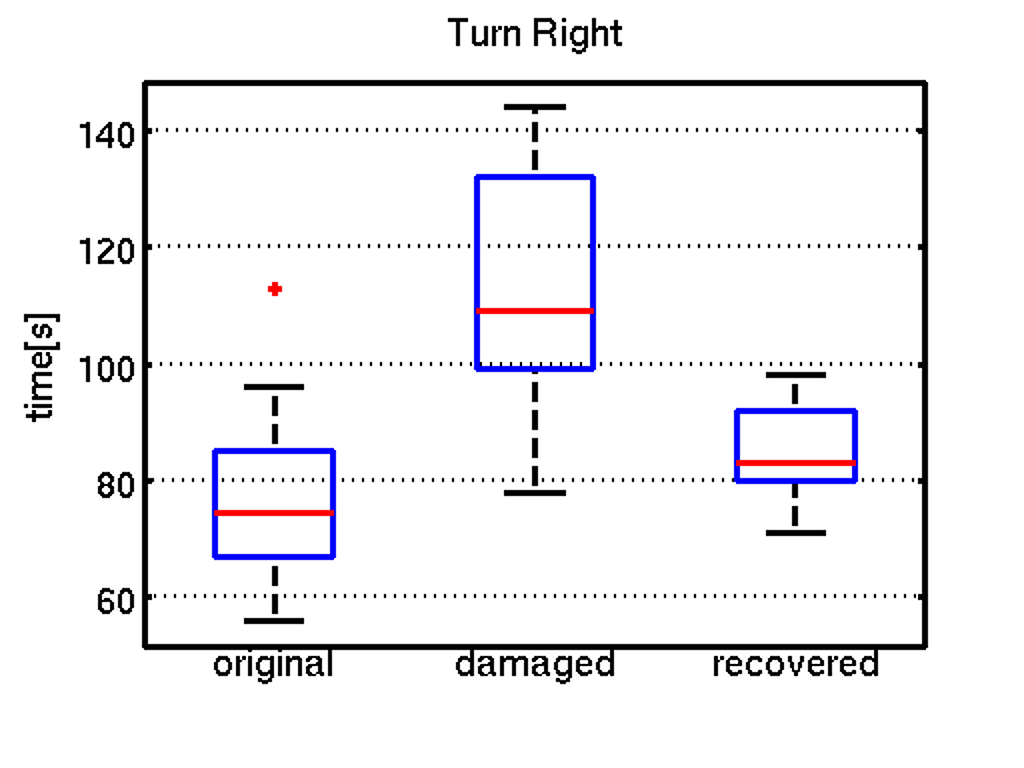
\includegraphics[width=\textwidth]{Files/Figures/box_recovery.png}
\caption[Box plot of turn right move during fault recovery]{Box plot of original, damaged and recovered \textit{Turn Right}. Median original:~74.5[s], Median damaged:~109[s], Median recovered:~83[s]}
\label{fig:box_recovery}
\endminipage\hfill
\end{figure}

\begin{table}
\centering
\renewcommand{\arraystretch}{1.0}
\begin{tabular}{rccc}
\hline
\# & Turn Left & Turn Right & Waypoints\\
 & [mm:ss.ss] & [mm:ss.ss] & [mm:ss.ss]\\
\hline
\rowcolor{Gray}
1 & 01:22.00 & 01:32.00 & 04:33.00\\
2 & 00:57.00 & 01:32.00 & 03:20.00\\
\rowcolor{Gray}
3 & 01:00.00 & 01:26.00 & \textit{N/A}\\
4 & 00:52.00 & 01:22.00 & \textit{N/A}\\
\rowcolor{Gray}
5 & \textit{N/A} & 01:19.00 & \textit{N/A}\\
6 & \textit{N/A} & 01:24.00 & \textit{N/A}\\
\rowcolor{Gray}
7 & \textit{N/A} & 01:20.00 & \textit{N/A}\\
8 & \textit{N/A} & 01:38.00 & \textit{N/A}\\
\rowcolor{Gray}
9 & \textit{N/A} & 01:22.00 & \textit{N/A}\\
10 & \textit{N/A} & 01:11.00 & \textit{N/A}\\
\hline
\textbf{Mean:} & \textbf{01:02.75} & \textbf{01:24.60} & \textbf{03:56.00}\\
\textbf{Max:} & 01:22.00 & 01:38.00 & \textit{N/A}\\
\textbf{Min:} & 00:52.00 & 01:11.00 & \textit{N/A}\\
\hline
\end{tabular}
\newline
\caption[Basic maneuvers performed after recovery]{Basic maneuvers performed after recovery left wing damage with updated control parameters.}
\label{tab:times-repaired}
\end{table}


\begin{figure}
\centering
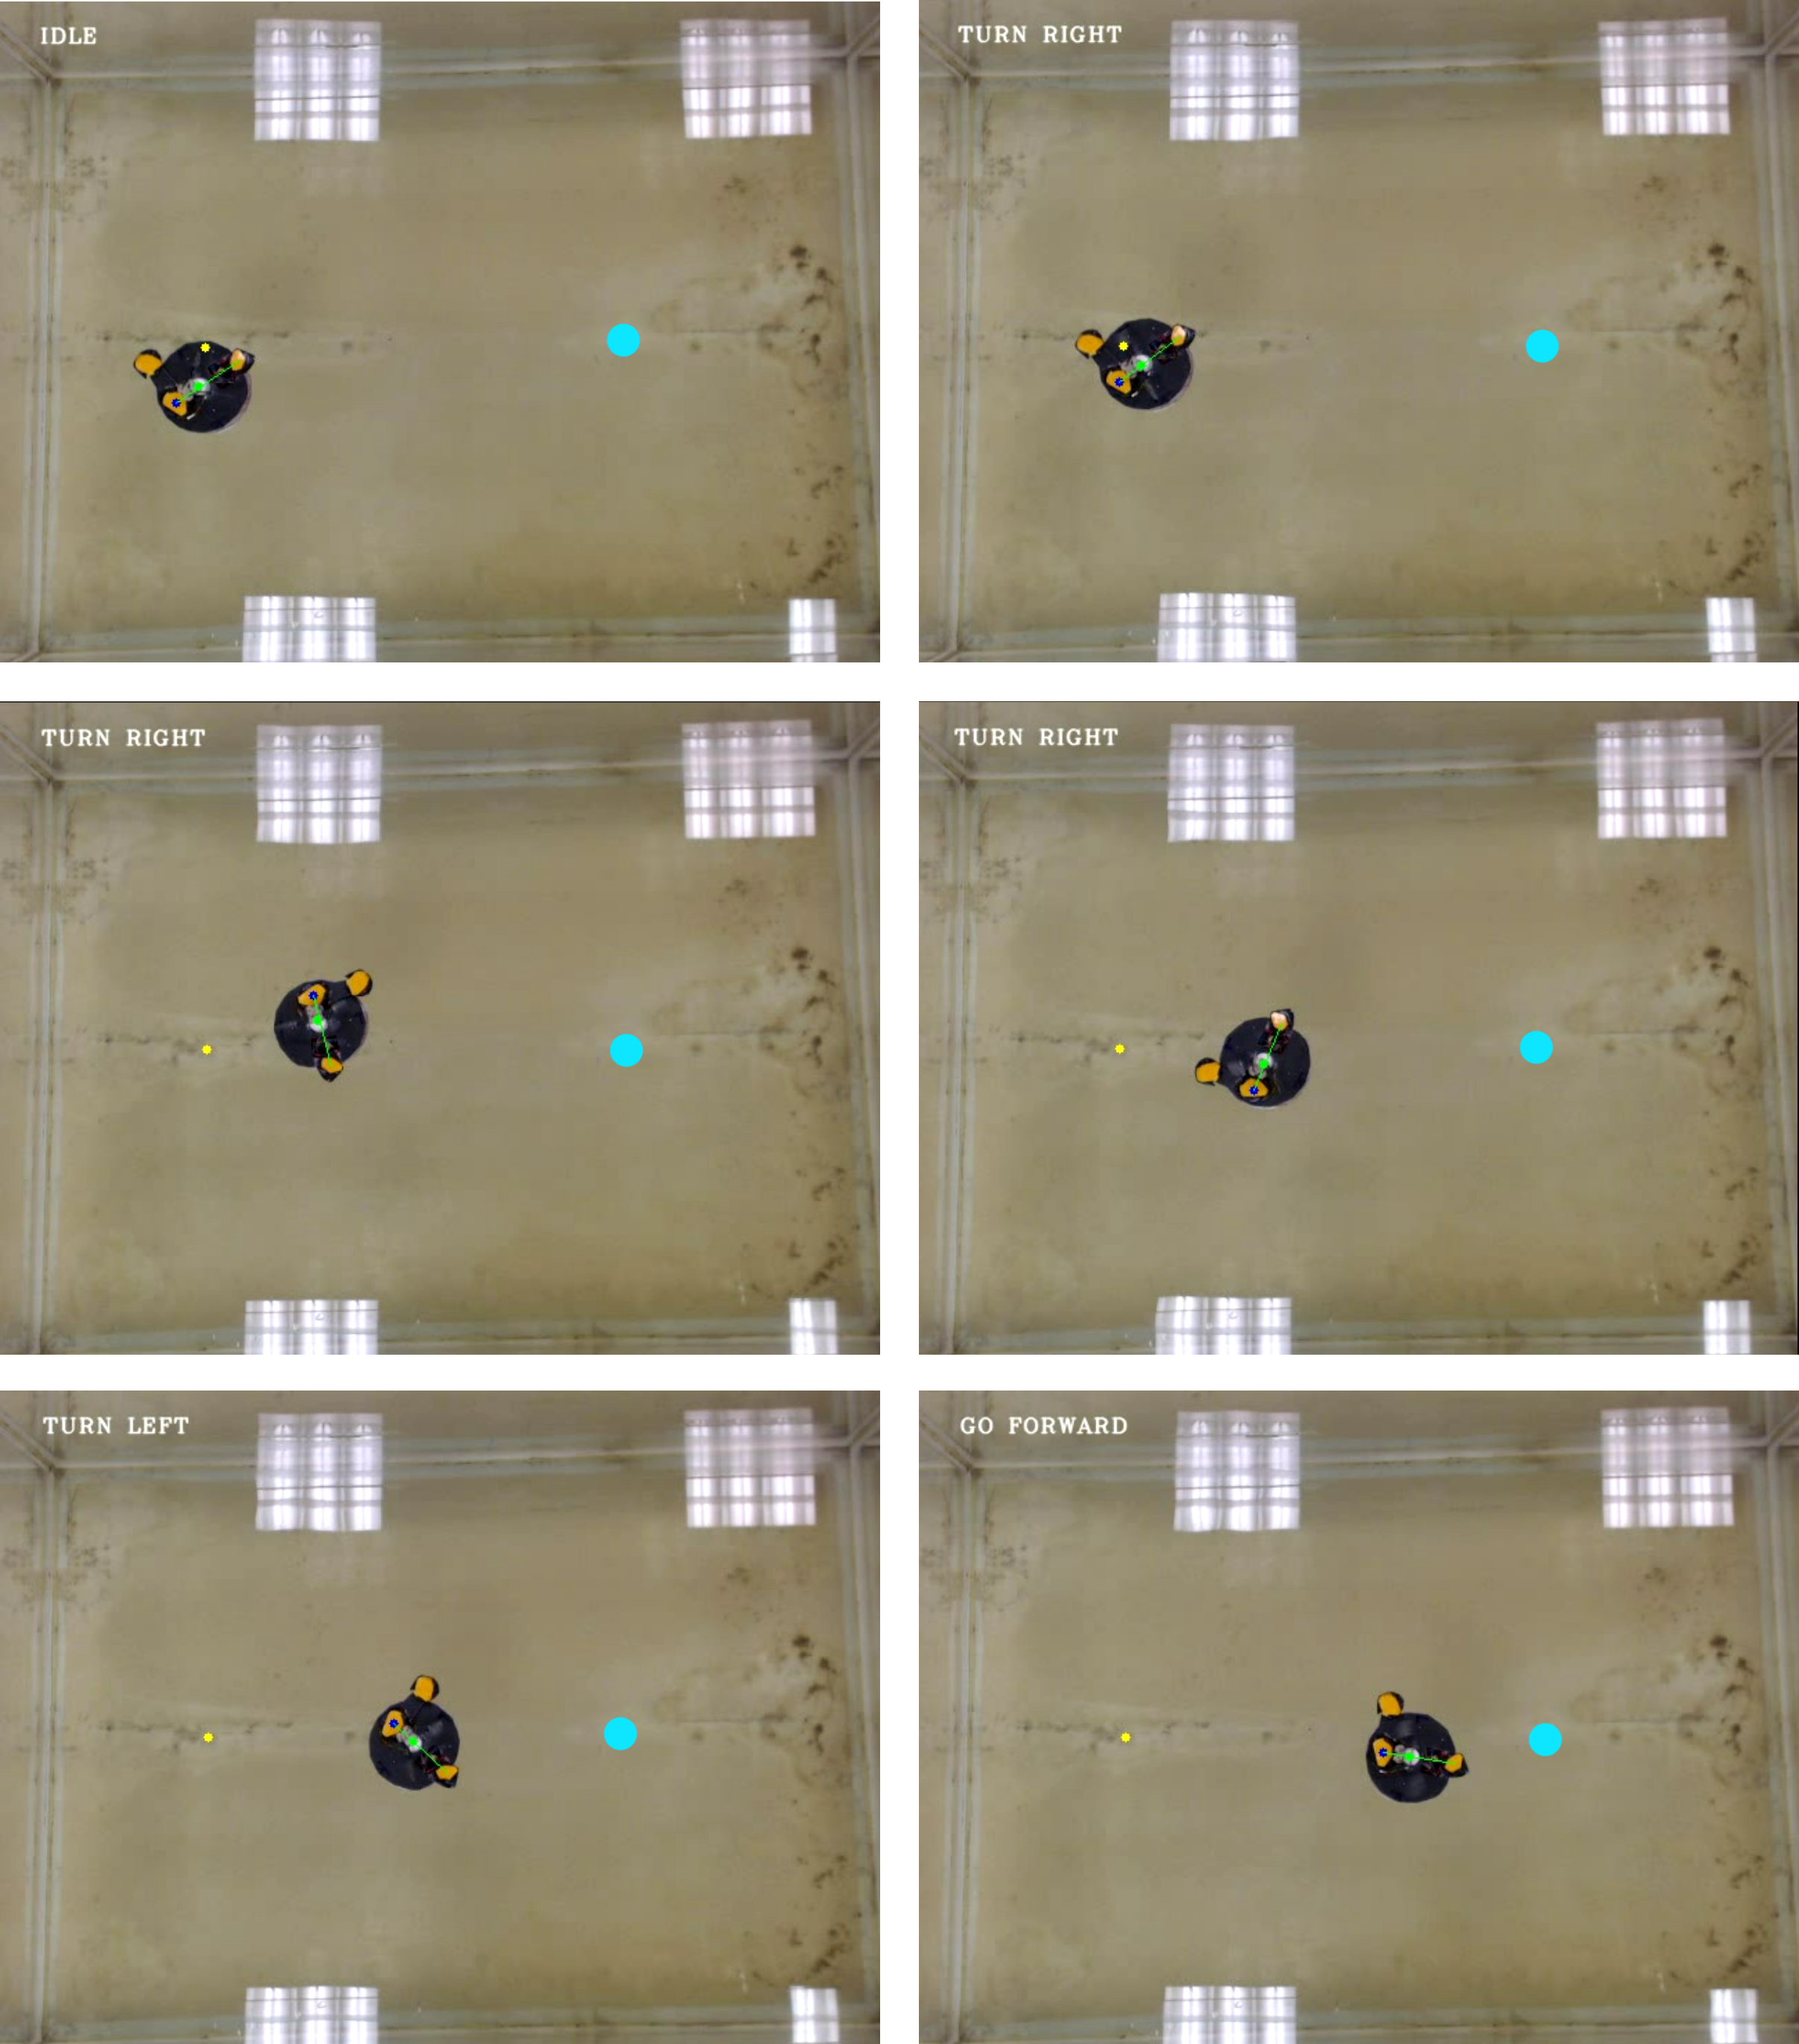
\includegraphics[width=\textwidth]{Files/Figures/fault_recovery.png}
\caption[Fault recovery example]{Fault recovery example. The obstacle is the green line located in the middle of the water tank, the waypoint the wehicle follows is marked light blue. \textit{Top left:} the vehicle is initializing its wings (takes around 30~sec at the beginning of each experiment), \textit{Top right:} the diagnostic agent initiates the diagnostics and starts a 360~deg right turn, \textit{Middle left:} diagnostics in progress, \textit{Middle right:} diagnostics was finished, the diagnostics agent found a presence of a fault and loaded the evolved fault-recovery control values, \textit{Bottom left:} the vehicle is progressing towards the second waypoint, \textit{Bottom right:} Final approach towards the waypoint}
\label{fig:fault_recovery_pics}
\end{figure}

\begin{figure}
\centering
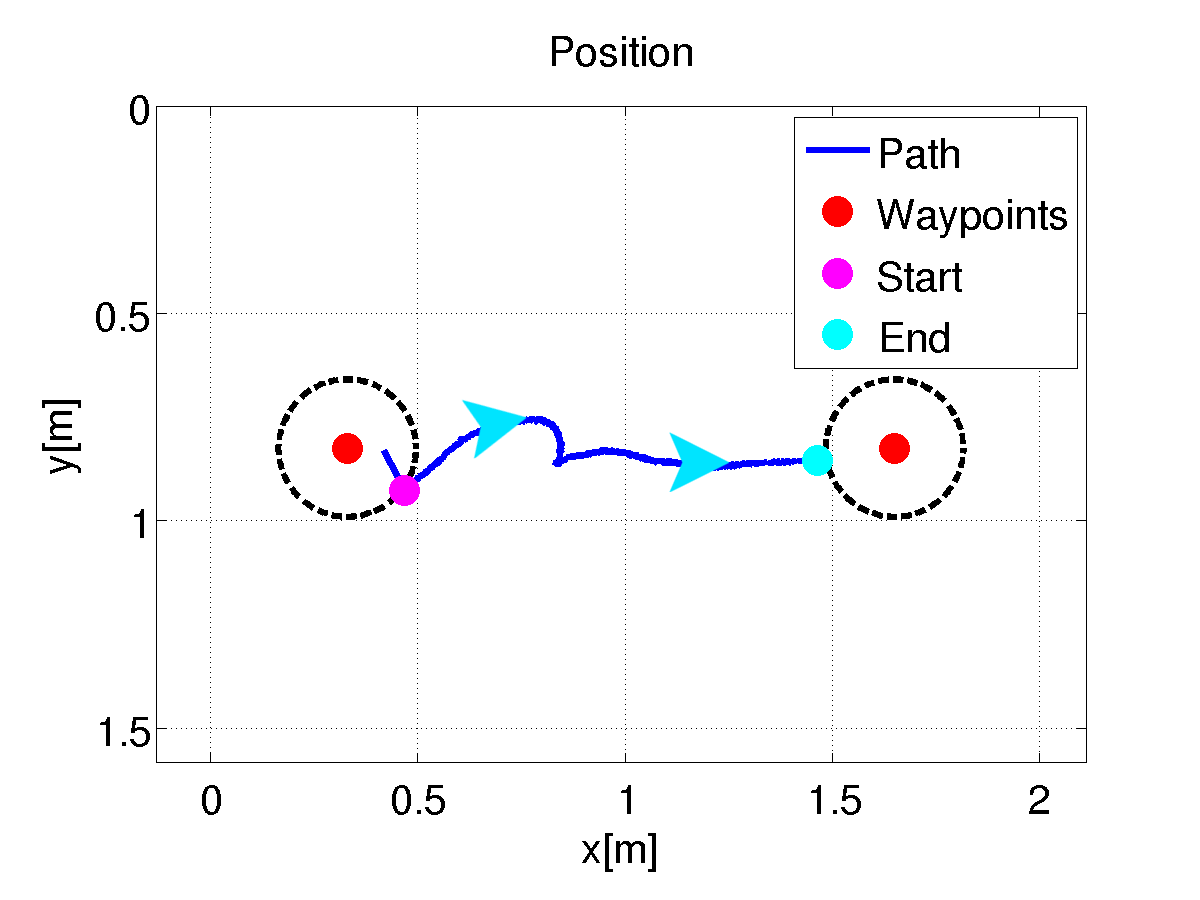
\includegraphics[width=0.8\textwidth]{Files/Figures/faultrec_2016-06-21_14-26-34-position.png}
\caption[Path travelled during fault recovery]{Path travelled during fault recovery maneuver from Figure~\ref{fig:obstacle_avoidance}. \textit{Purple:} start position, \textit{Light blue:} end position, \textit{Green line:} the obstacle, \textit{Blue arrows:} indicate the orientation of the vehicle}
\label{fig:fault_recovery_path}
\end{figure}

\begin{figure}
\centering
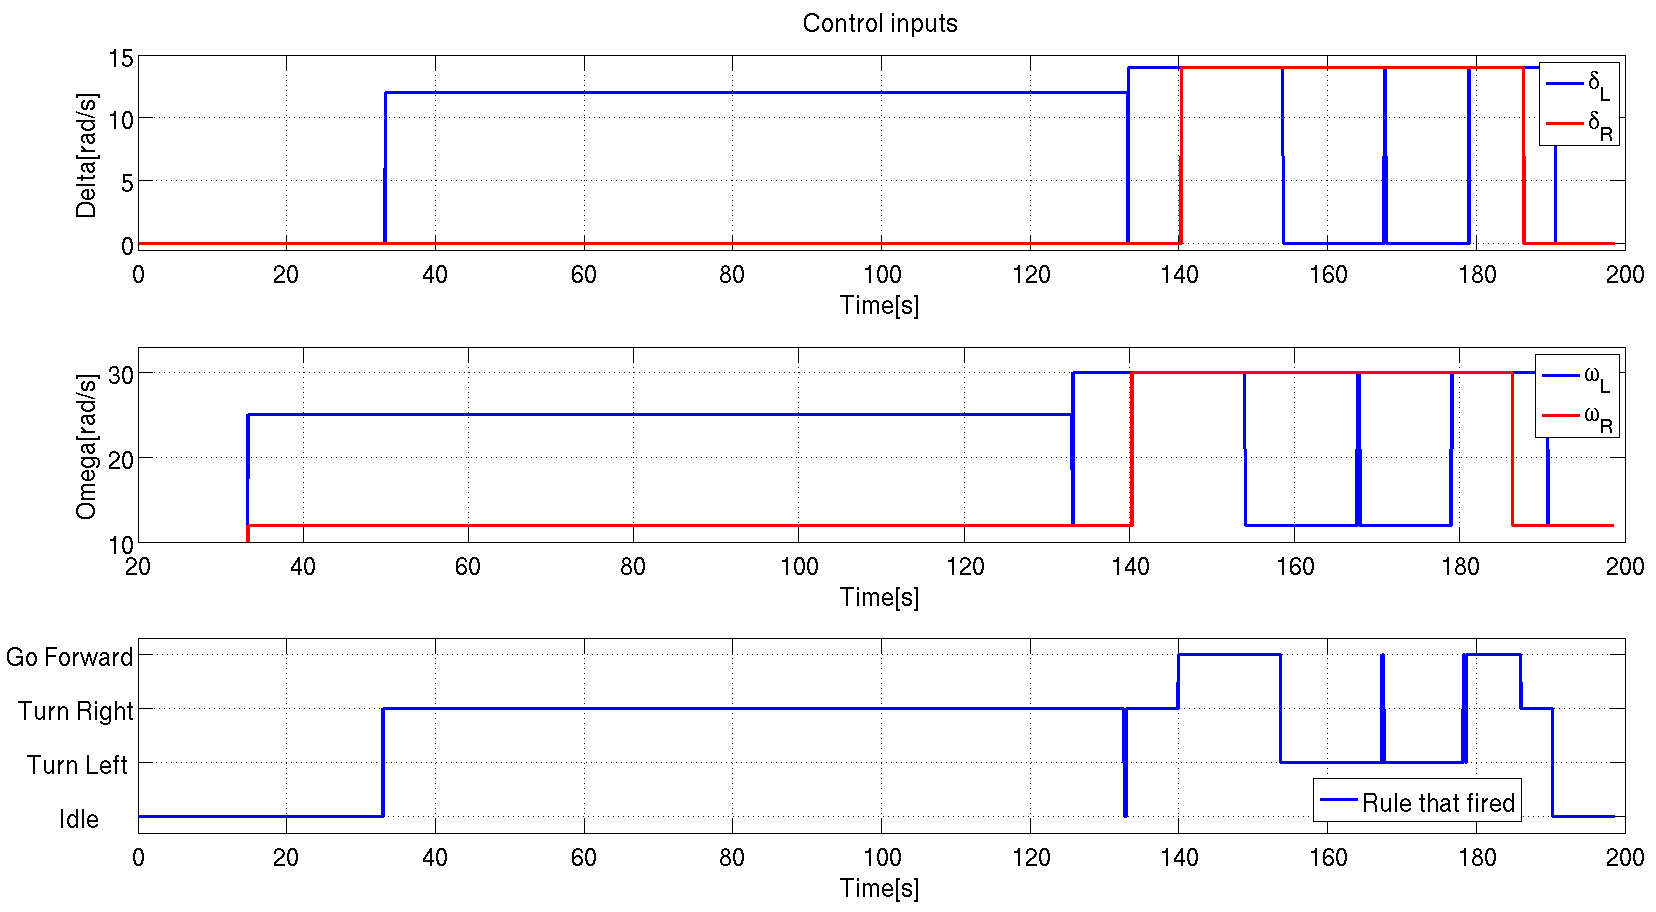
\includegraphics[width=\textwidth]{Files/Figures/faultrec_2016-06-21_14-26-34_control_inputs.png}
\caption[Control inputs during fault recovery]{Control inputs during fault recovery. \textit{Top:} $\delta$ values, \textit{Middle:} $\omega$ values, \textit{Bottom:} rule that fired. Note the 30 second initialization period at the beginning of the experiment (rule: \textit{Idle}), and the diagnostics phase with \textit{Turn Right} command.}
\label{fig:fault_recovery_control_input}
\end{figure}


\begin{figure}
\centering
\minipage{0.49\textwidth}
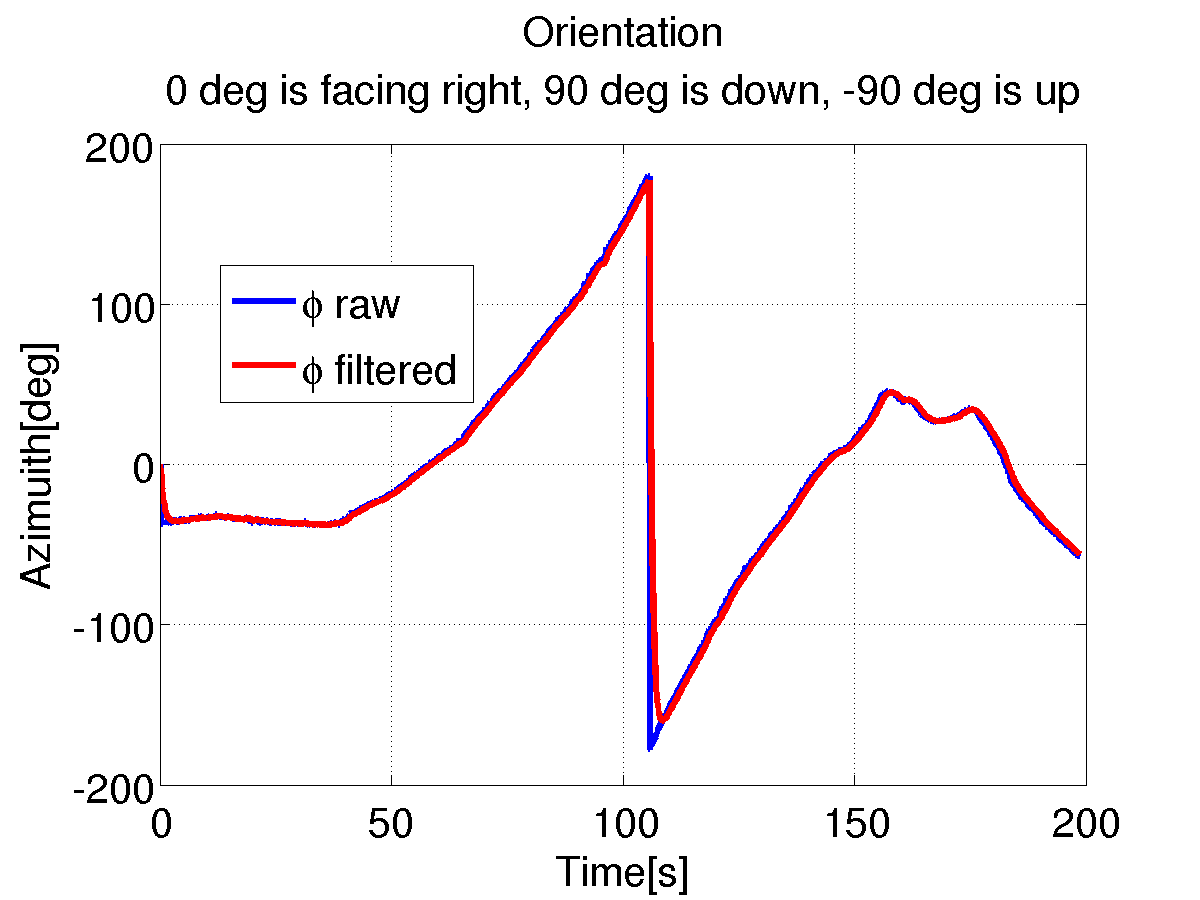
\includegraphics[width=\textwidth]{Files/Figures/faultrec_2016-06-21_14-26-34-orientation.png}
\caption[Orientation during fault recovery]{Heading of the vehicle during fault recovery. Note the wrap-around at $\pm180$~deg. 0~deg is in the direction of positive x-axis, $\pm180$~deg is in the direction of negative x-axis. The values were filtered with an exponential moving average low-pass filter with $\alpha=0.05$}
\label{fig:fault_recovery_orientation}
\endminipage\hfill
\minipage{0.49\textwidth}
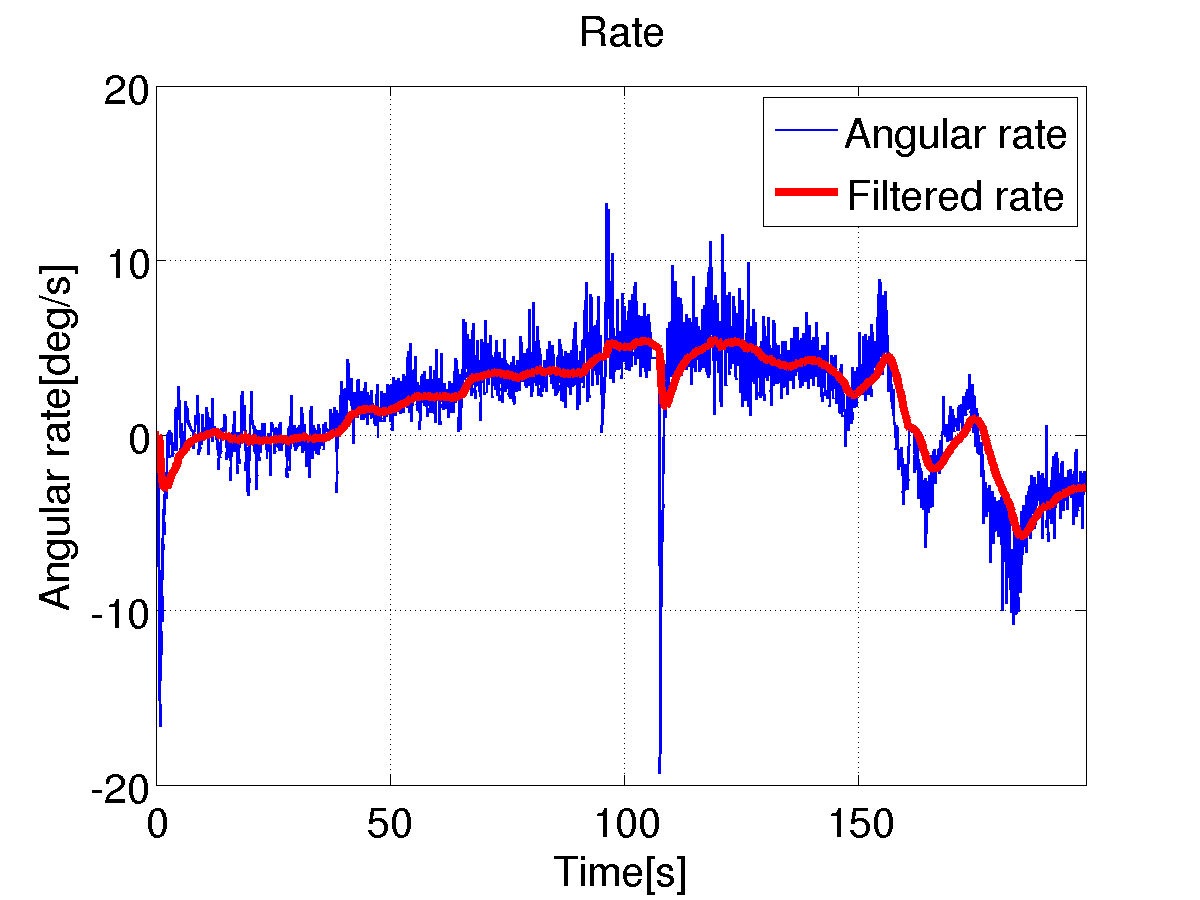
\includegraphics[width=\textwidth]{Files/Figures/faultrec_2016-06-21_14-26-34-ang_rate.png}
\caption[Angular rate during fault recovery]{Angular rate of the vehicle's heading during fault recovery. The values were filtered with an exponential moving average low-pass filter with $\alpha=0.05$. The large peak is a residual from a wrap-around at $\pm180$~deg.\newline.}
\label{fig:fault_recovery_ang_rate}
\endminipage\hfill
\end{figure}

\newpage

\section{Obstacle Avoidance}
\label{sec:obstacle-avoidance}
During the experiments it became apparent that a modification of the rule base from Table~\ref{tab-subsum} is necessary. Specifically, the rule number 1: \textbf{if} outside perimeter \textbf{then} \textit{Hard right turn} never occurs, because the robot cannot physically get outside the perimeter (there are walls in the water tank). Limiting the size of the operating area, so the robot is not allowed to hit the walls, is impractical, because of the extra space limitation. More practical response would be \textit{avoid hitting the wall} or more generally \textit{avoid obstacle}. \textit{Hard right turn} is also not distinguishable from a \textit{Partial right turn}, because the vehicle is already operating at its maximal capability, and is turning as fast as possible. A modified rule base that contains these changes is shown in Table~\ref{tab-subsum-modified}.


The \textit{Avoid Obstacle} routine needs to be more complex than the other rule consequents. In this case the position of the obstacle is explicitly known, which is sufficient if we want the vehicle to avoid walls of the water tank and/or obstacles that are imposed in the water. The routine goes is summarized in Algorithm~\ref{algo:oa}


\begin{table}
\centering
\renewcommand{\arraystretch}{1.7}
\begin{tabular}{>{\small}c>{\small}l}
\hline
Layer & Behavior\\
\hline
\rowcolor{Gray}
6 & \textbf{if} true \textbf{then} \textit{Idle} \\
5 & \textbf{if} heading left \textbf{then} \textit{Partial right turn}\\
\rowcolor{Gray}
4 & \textbf{if} heading right \textbf{then} \textit{Partial left turn}\\
3 & \textbf{if} heading at waypoint \textbf{then} \textit{Move forward}\\
\rowcolor{Gray}
2 & \textbf{if} at waypoint $W_j$ \textbf{then} Get new waypoint $W_{j+1}$\\
1 & \textbf{if} obstacle ahead \textbf{then} \textit{Avoid Obstacle}\\
\hline
\end{tabular}
\newline
\caption[Modified Controller agent subsumption architecture]{Modified Scheme of Controller agent subsumption architecture with updated rule for Layer 1 (Layer 1 has the highest priority).}
\label{tab-subsum-modified}
\end{table}


\begin{algorithm}
\caption{Updated Obstacle Avoidance routine}
\label{algo:oa}
\begin{algorithmic}
\IF{$WP_2$ behind the obstacle}
\STATE move $WP_{tmp}$ in front of the obstacle on the $|WP_1,WP_2|$ line;
\ENDIF
\WHILE{!wp\_reached($WP_{tmp}$)}
\STATE wait;
\ENDWHILE
\STATE shift $WP_{tmp}$ right (vehicle side) until after the obstacle ends;
\WHILE{!wp\_reached($WP_{tmp}$)}
\STATE wait;
\ENDWHILE
\STATE shift $WP_{tmp}$ forward (vehicle side) behind the obstacle;
\WHILE{!wp\_reached($WP_{tmp}$)}
\STATE wait;
\ENDWHILE
\STATE shift $WP_{tmp}$ left (vehicle side) on the $|WP_1,WP_2|$ line;
\WHILE{!wp\_reached($WP_{tmp}$)}
\STATE wait;
\ENDWHILE
\STATE follow $WP_2$ \& \textbf{return};
\end{algorithmic}
\end{algorithm}


where $WP_1$ is the initial waypoint, $WP_2$ is the final waypoint, and $WP_{tmp}$ is an intermittent waypoint that the vehicle follows while avoiding the obstacle. An example will better explain this - a run with an obstacle in the middle of the water tank is described in Figure~\ref{fig:obstacle_avoidance}, and Figure~\ref{fig:obstacle_avoidance_path} shows the path the vehicle travelled. The most common rule is \textit{Turn Right} and \textit{Go Forward}. Figures~\ref{fig:obstacle_avoidance_orientation} and ~\ref{fig:obstacle_avoidance_ang_rate} show the heading and the angular rate of the vehicle during the experiment. As can be seen, the vehicle was able to successfully avoid the obstacle.

This obstacle avoidance routine can be improved, because at the moment it covers only cases where a waypoint is behind the obstacle (so going straight ahead is not possible). However, our experience from conducting the experiments has shown that in order to avoid occasionally hitting the walls of the water tank, a more nimble vehicle with more control authority is needed. For example, in several occasions the control system was issuing the correct commands to avoid hitting the wall (e.g. \textit{Partial right turn}), but the vehicle already had too much momentum from the previous movement that it couldn't be turned and stopped in time before the collision. Other example included improper initialization of the vehicle, and consequent malfunction of the control system. In both cases a better obstacle avoidance routine wouldn't have helped.

\begin{figure}
\centering
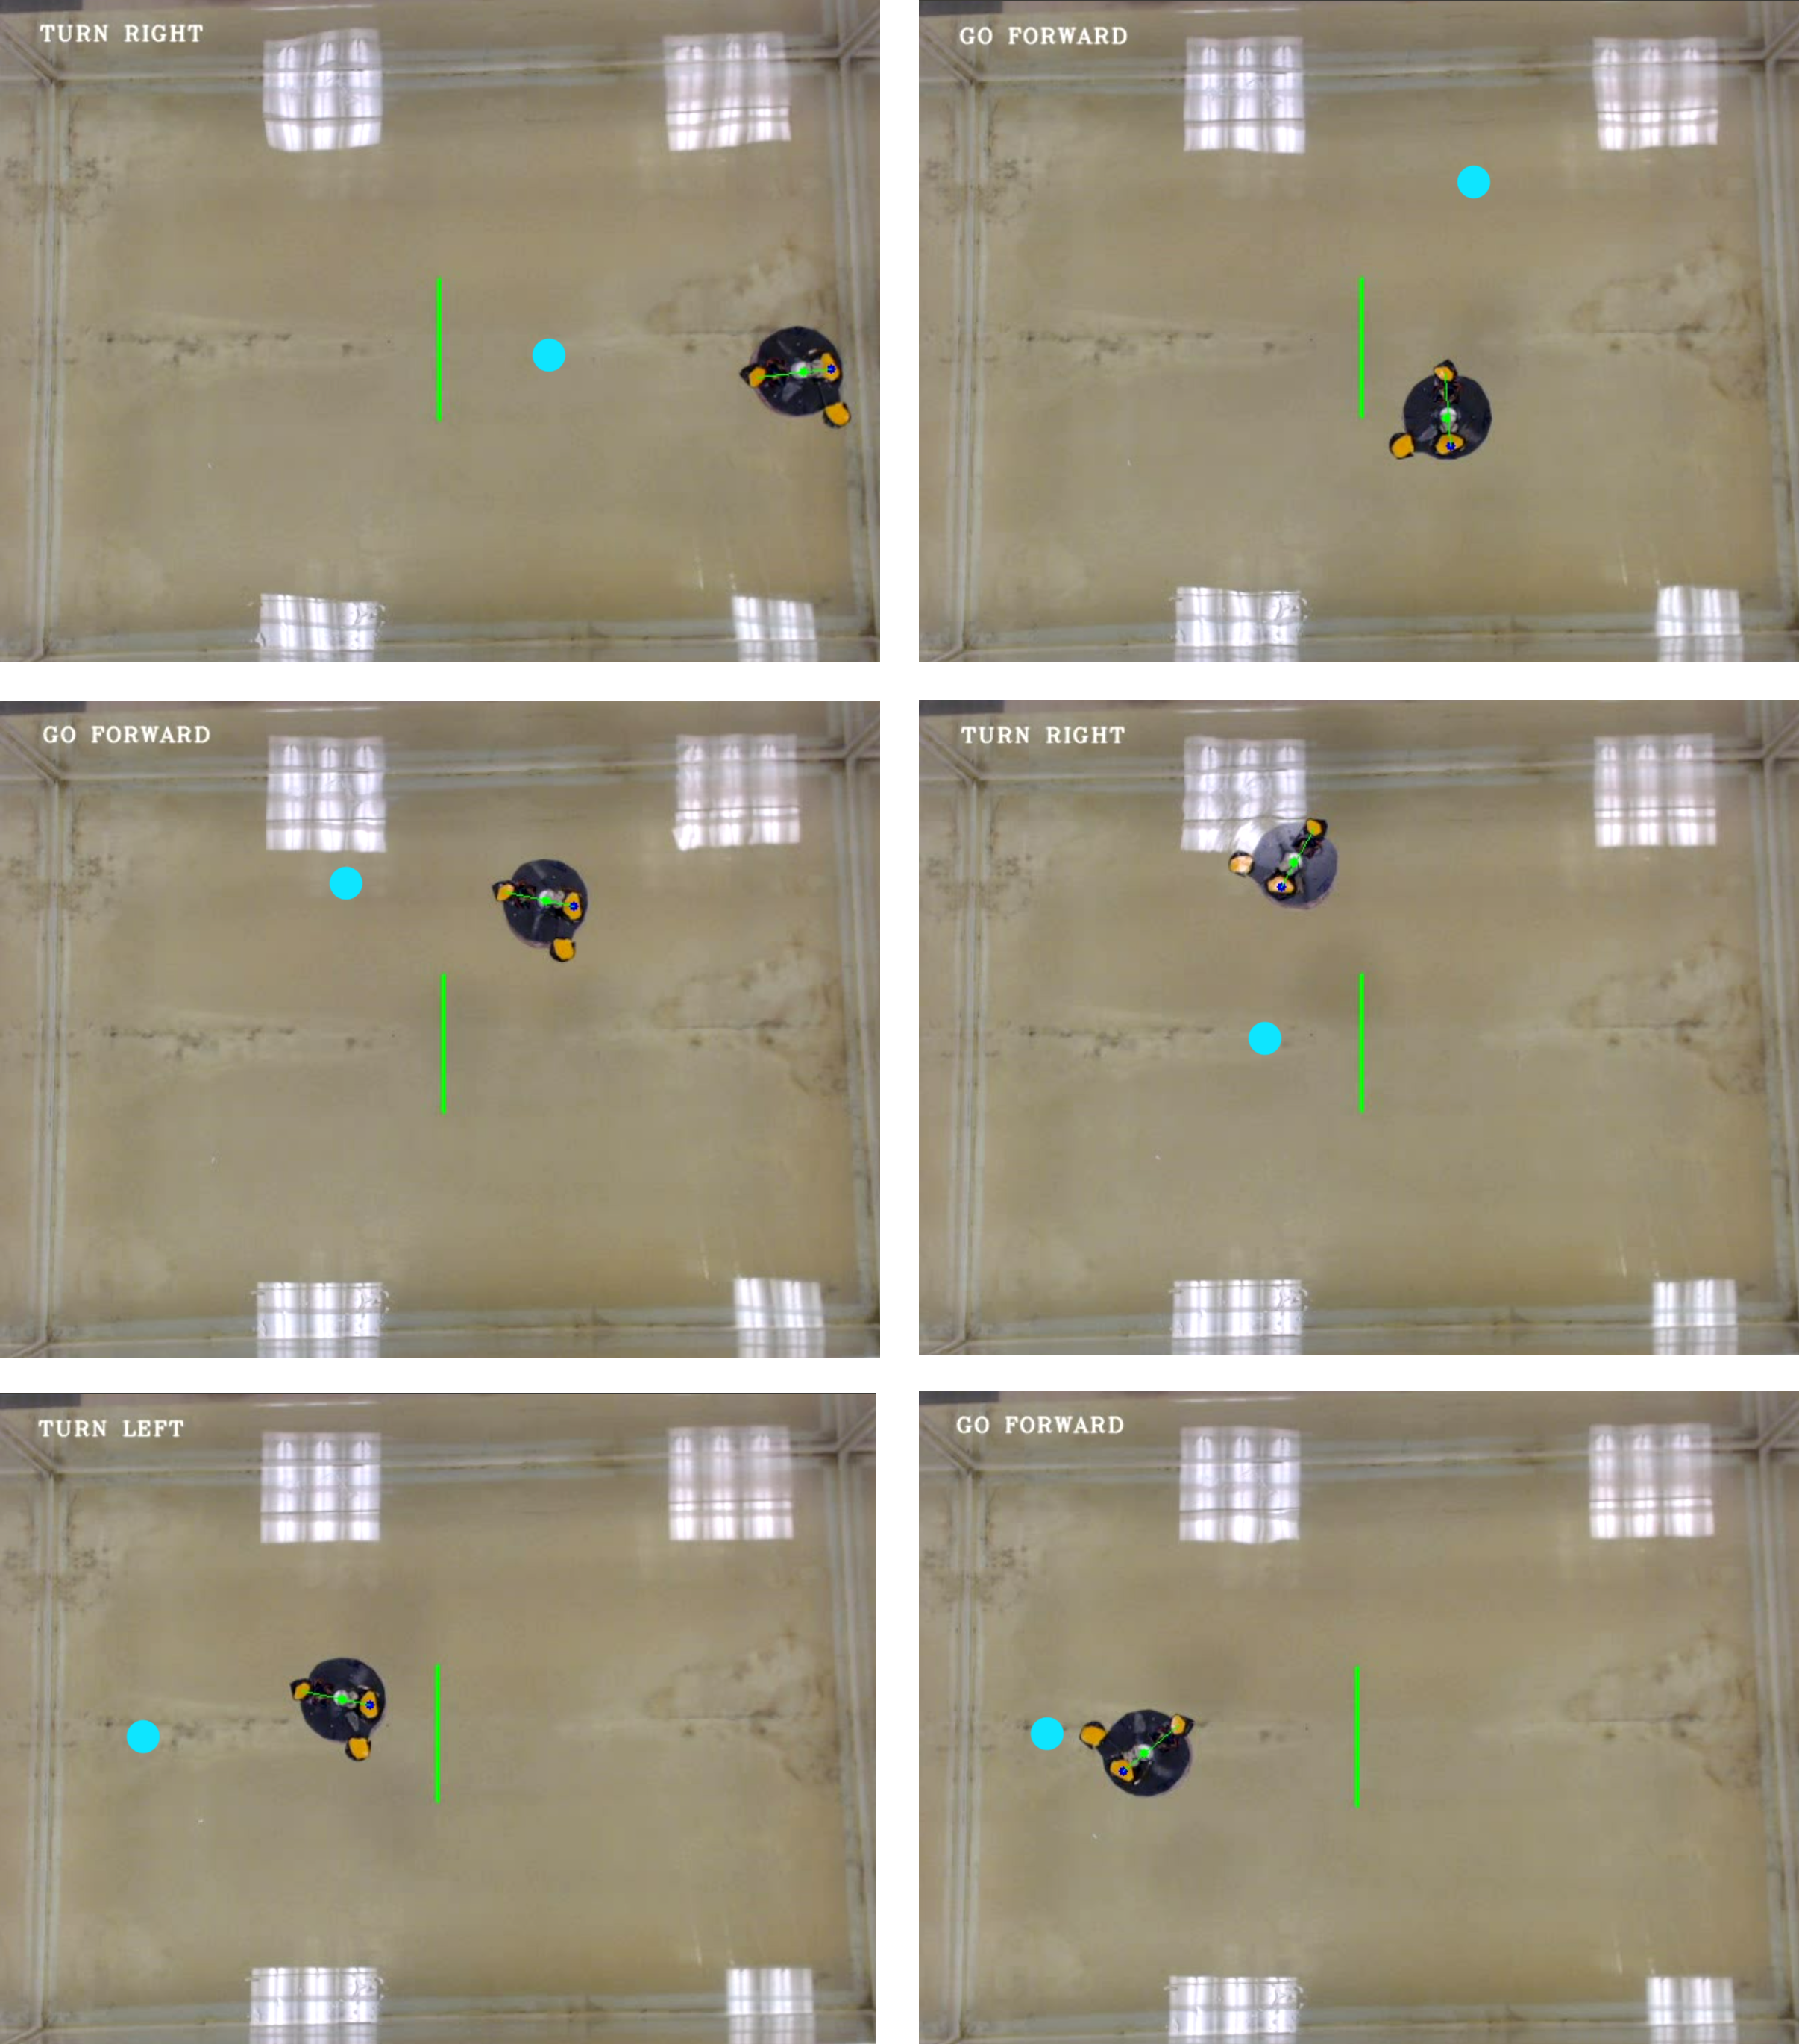
\includegraphics[width=\textwidth]{Files/Figures/obstacle_avoidance.png}
\caption[Obstacle avoidance example]{Obstacle avoidance example. The obstacle is the green line located in the middle of the water tank, the waypoint the wehicle follows is marked light blue. \textit{Top left:} vehicle starting at $WP_1$, moving towards the obstacle. \textit{Top right:} vehicle reached $WP_{tmp}$ in front of the obstacle and moved it above the obstacle. \textit{Middle left:} $WP_{tmp}$ is behind the obstacle. \textit{Middle right:} $WP_{tmp}$ is on the $|WP_1,WP_2|$ line. \textit{Bottom left:} end of \textit{Avoid Obstacle} routine, the vehicle follows $WP_2$. \textit{Bottom right:} the vehicle is about to reach $WP_2$}
\label{fig:obstacle_avoidance}
\end{figure}

\begin{figure}
\centering
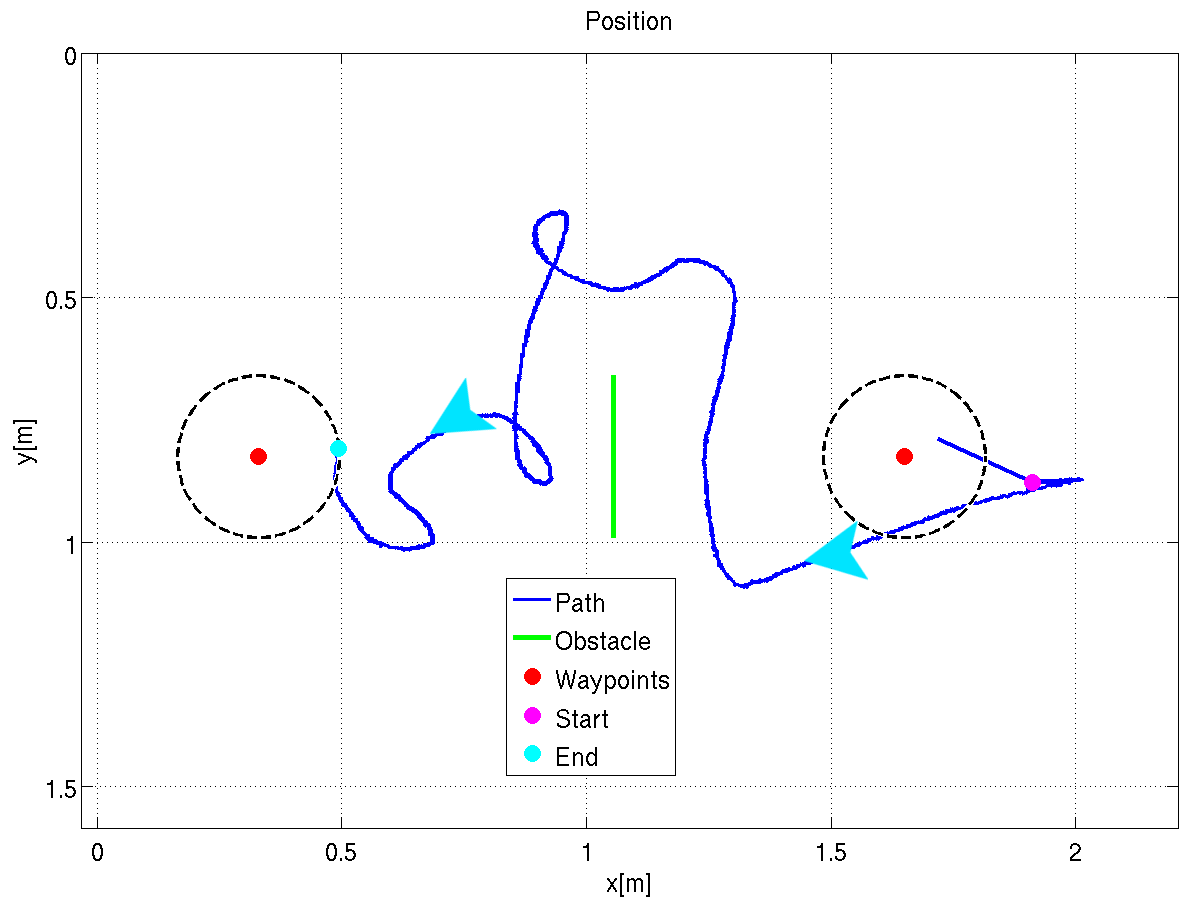
\includegraphics[width=0.8\textwidth]{Files/Figures/oavoidance_2016-05-09_12-04-15-position.png}
\caption[Path travelled during obstacle avoidance]{Path travelled during obstacle avoidance maneuver from Figure~\ref{fig:obstacle_avoidance}. \textit{Purple:} start position, \textit{Light blue:} end position, \textit{Green line:} the obstacle, \textit{Blue arrows:} indicate the orientation of the vehicle}
\label{fig:obstacle_avoidance_path}
\end{figure}

\begin{figure}
\centering
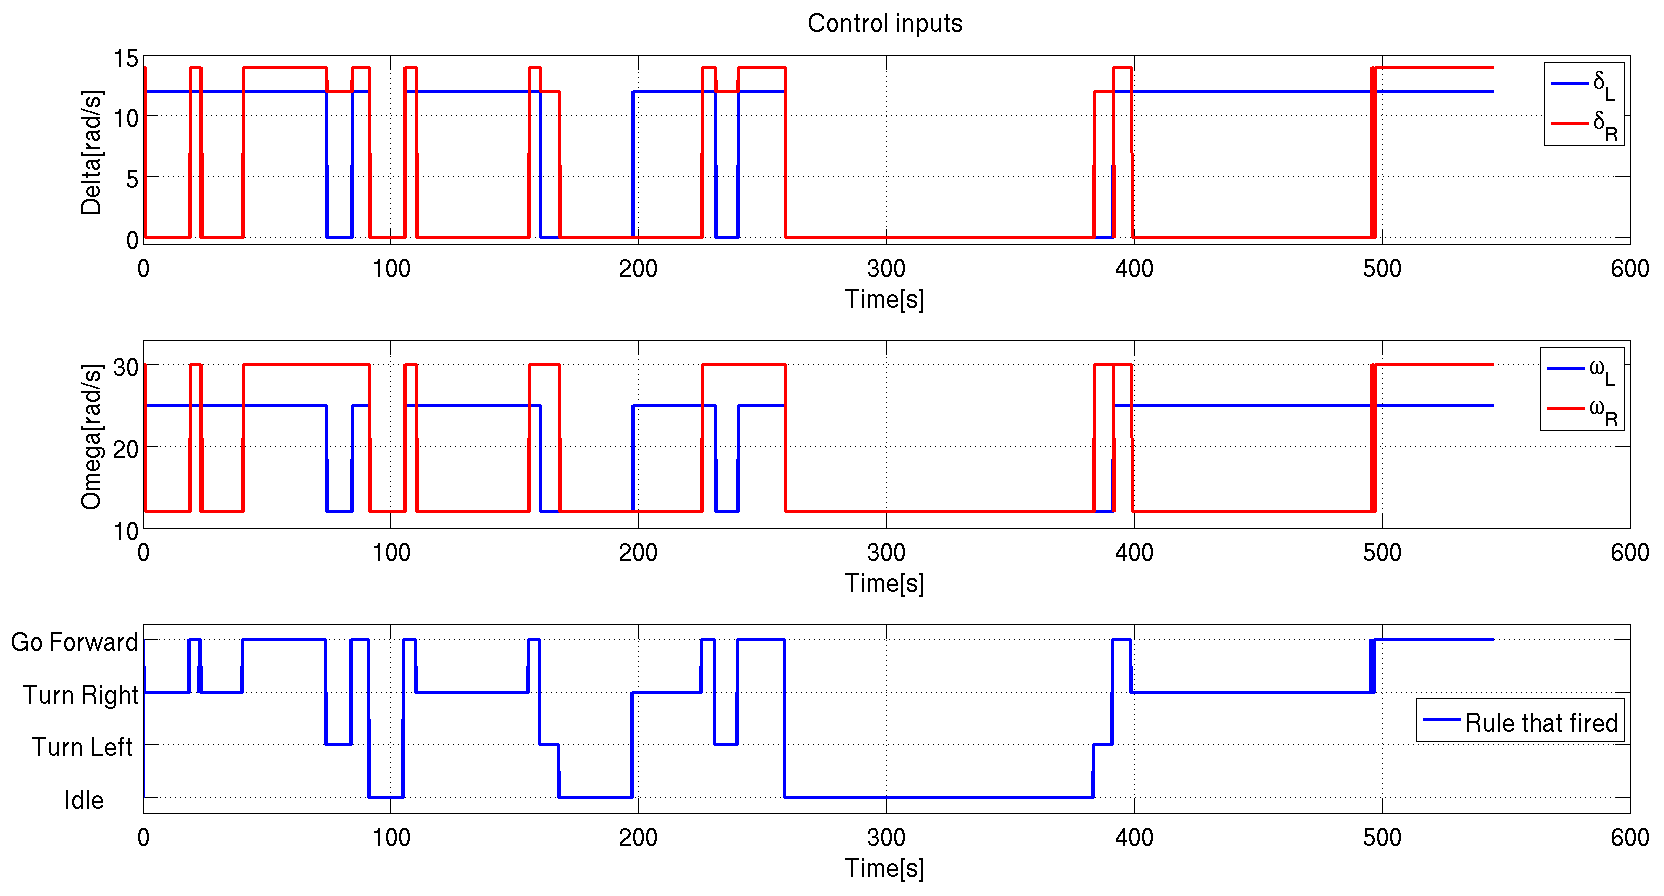
\includegraphics[width=\textwidth]{Files/Figures/oavoidance_2016-05-09_12-04-15-control-inputs.png}
\caption[Control inputs during obstacle avoidance]{Control inputs during obstacle avoidance. \textit{Top:} $\delta$ values, \textit{Middle:} $\omega$ values, \textit{Bottom:} rule that fired. The large segment of \textit{Idle} in the middle of the experiment is caused by a momentary loss of tracking of the algorithm.}
\label{fig:obstacle_avoidance_control_input}
\end{figure}

\begin{figure}
\centering
\minipage{0.49\textwidth}
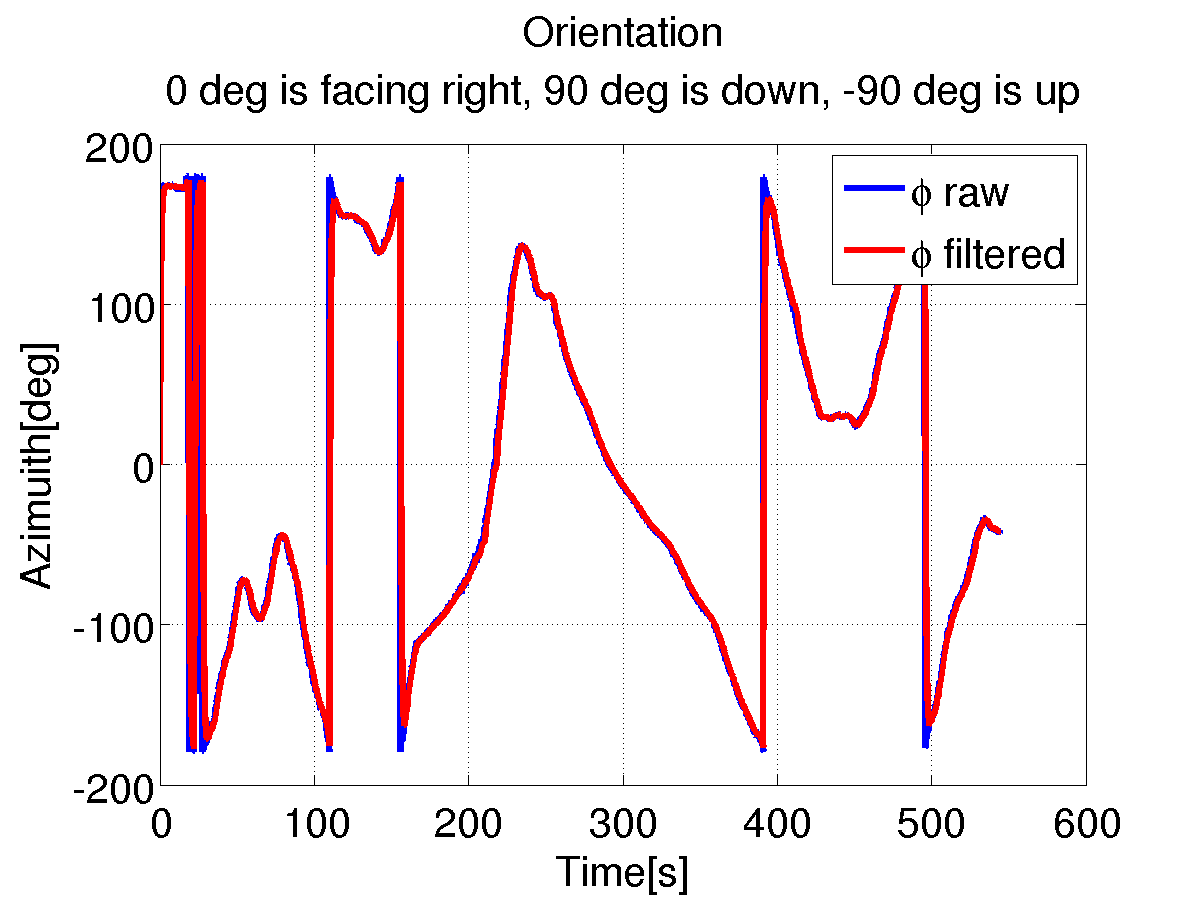
\includegraphics[width=\textwidth]{Files/Figures/oavoidance_2016-05-09_12-04-15-orientation.png}
\caption[Orientation during obstacle avoidance]{Heading of the vehicle during obstacle avoidance. Note the wrap-around at $\pm180$~deg. 0~deg is in the direction of positive x-axis, $\pm180$~deg is in the direction of negative x-axis. The values were filtered with an exponential moving average low-pass filter with $\alpha=0.05$}
\label{fig:obstacle_avoidance_orientation}
\endminipage\hfill
\minipage{0.49\textwidth}
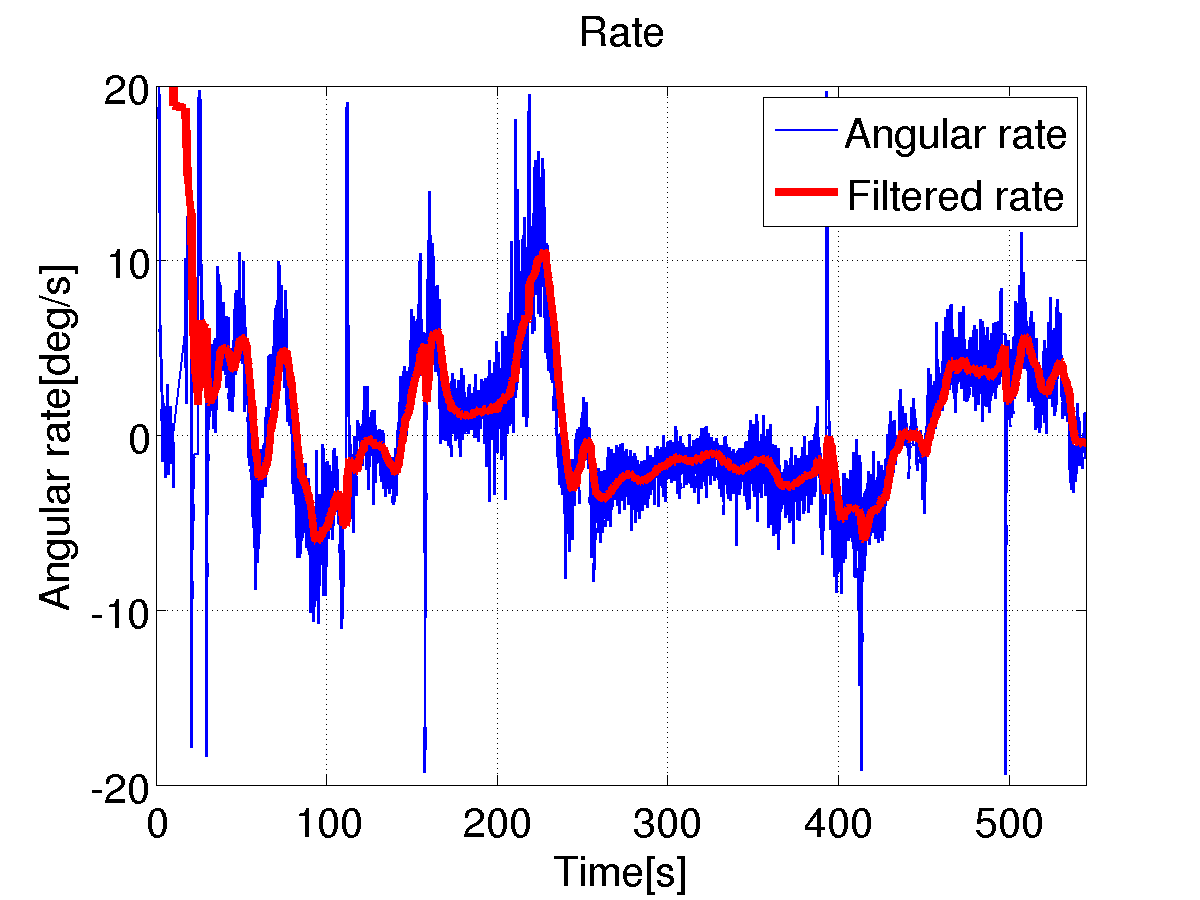
\includegraphics[width=\textwidth]{Files/Figures/oavoidance_2016-05-09_12-04-15-ang_rate.png}
\caption[Angular rate during obstacle avoidance]{Angular rate of the vehicle's heading during obstacle avoidance. The values were filtered with an exponential moving average low-pass filter with $\alpha=0.05$ The peaks are residuals from wrap-arounds at $\pm180$~deg.\newline}
\label{fig:obstacle_avoidance_ang_rate}
\endminipage\hfill
\end{figure}
%\vspace*{3in} % optional to align figures?

\newpage

\section{Summary}
%\label{sec:autonomous-mission}
In this chapter we demonstrated a successful implementation of the MAS from Chapter~\ref{ch:approach} and the EA for determining the values of control parameters $\delta$ and $\omega$. We have shown that the vehicle is capable of autonomous waypoint following, which was repeated multiple times, as well as fault detection and recovery - which was demonstrated with a damaged left wing. On top of that, we updated the rule base (see Tables~\ref{tab-subsum} and~\ref{tab-subsum-modified}) to better suite our needs, and implemented obstacle avoidance routine. The implications of this work and a conclusion of our efforts is discussed in the next chapter.